%\documentclass[handout]{beamer}
\documentclass{beamer}

\usepackage{color}
\usepackage{beamerthemesplit}
\usepackage[utf8]{inputenc}

%\usetheme{Malmoe}
%\usetheme{CambridgeUS}
%\usetheme{Hannover}

% Tema Simple
\usetheme[height=0.35cm]{Madrid}

% El que uso habitualmente:
%\usetheme[height=0.7cm]{Rochester}

% A dark look
%\usecolortheme{beetle}
\usecolortheme{dolphin}

\setbeamertemplate{navigation symbols}{} 

%\usepackage{wrapfig}
\setbeamercovered{transparent}

\usepackage{geometry}
%\geometry{landscape}
\usepackage{multimedia}
\usepackage{verbatim}
\usepackage{bm}%bold matH

%\usepackage{shade}
\usepackage{fancybox}
 
\usepackage{amssymb}


% Defino clases de secciones en ESPAÑOL
\def\chaptername{Cap\'\i tulo}
\def\abstractname{Resumen}
\def\contentsname{Contenidos}
\def\bibname{Bibliograf\'\i a}
\def\appendixname{Ap\'endice}
\def\tablename{\textbf{Tabla}}
\def\figurename{\textbf{Figura}}
%\usepackage[dvips]{graphics,color,epsfig}
%\usepackage{pst-all}
%\usepackage{pstricks}
%\topmargin=-2cm  

% Defino formatos
\def\titulo#1{\frametitle{{\ \hfill {\bf #1}}}}
\def\figu#1{\shadowbox{#1}}

\def\Eeuv{E_{\rm{EUV}}}
\def\Ewl{E_{\rm{WL}}}
\def\AvgNE2{\left<N_e^2\right>}
\def\AvgNe{\left<N_e\right>}
\def\SigmaNe{\sigma_{Ne}}
\def\VarNe{\rm{Var}N_e}
\def\AvgTe{\left<T_e\right>}
\def\SigmaTe{\sigma_{Te}}


%EStilo
%\input{epsf.sty}

%Paquetes a utilizar

%\usepackage{amssymb} % Math
%\usepackage{graphicx}
%\usepackage{float}
%%\usepackage{wrapfig}
%%\usepackage{deluxetable}

\pagenumbering{arabic}
%\usepackage[dvips]{graphics,color}
%\usepackage{natbib}
%\usepackage{amssymb} % Math
%\usepackage{amsmath} % Math
%%\usepackage{dsfont} % Math
%\usepackage{float}
%\usepackage{graphicx}
%%\usepackage{wrapfig}
%\usepackage{pst-all}
%%\usepackage{multirow} % Multi filas

%Separacion silabica:
%%\usepackage[T1]{babel} % silabas y hyphenation
%\hyphenation{e-vi-den-cia}
%\hyphenation{an-te-rio-res}

% Control de Márgenes

%-------------------- Comandos de los autores ----------------------------

% Nombres de Journals
\newcommand{\araa}{Annu. Rev. Astron. Astrophys.}
\newcommand{\solphys}{Solar Phys.}
\newcommand{\aapr}{Astron. Astrophys. Rev.}
\newcommand{\aaps}{Astron. Astrophys. Sup. Ser.}
\newcommand{\jastp}{Jour. Atmos. Solar-Terrestrial Phys.}
\newcommand{\pasj}{Pub. Astron. Soc. Japan}
\newcommand{\etal}{et al.\ }
\newcommand{\ha}{H$\alpha$ }
\newcommand{\aap}{Astron. \& Astrophys.}
\newcommand{\apjs}{Astrophys J. Sup.}
\newcommand{\jgr}{Journal of Geophys. Res.}
\newcommand{\grl}{Geophys. Res. Let.}
\newcommand{\pre}{Physical Rev. E}
\newcommand{\adv}{Adv. in Space Res.}
\newcommand{\SpaceS}{Space Science Reviews}
\newcommand{\planss}{Planet. Space Sci.}
\newcommand{\nat}{Nature}
\newcommand{\apj}{The Astrophysical Journal}
\newcommand{\apjS}{The Astrophysical Journal Supplement}
\newcommand{\apjl}{The Astrophysical Journal Letters}
\newcommand{\mnras}{MNRAS}
\newcommand{\pasp}{Publications of the Astronomical Society of the Pacific}
\newcommand{\apss}{Astrophys. Space Sci.}

% Formato
\def\salto{\vskip 0.3cm}
\def\mediosalto{\vskip 0.15cm}

% Math:
\def\deg{$^\circ$}
\def\rsun{R$_{\odot}$}
\def\bB{\mathbf{B}}
\def\bE{\mathbf{E}}
\def\dpar#1#2{\frac{\partial#1}{\partial#2}}
%color:
\def\red#1{{\textcolor{red}{#1}}}
\def\azul#1{{\textcolor{blue}{#1}}}

\def\Figura#1{Figura \ref{#1}}
\def\Figuras#1#2{Figuras \ref{#1} a \ref{#2}}
\def\Figurasy#1#2{Figuras \ref{#1} y \ref{#2}}
\def\Tabla#1{Tabla \ref{#1}}
\def\Eq#1{Ecuaci\'on (\ref{#1})}
\def\Eqs#1#2{Ecuaciones (\ref{#1})-(\ref{#2})}
\def\Eqn#1{Ecuaci\'on (\ref{#1})}
\def\eqsy#1#2{Ecuaciones (\ref{#1}) y (\ref{#2})}

\def\exp{{\rm exp}}
\def\ln{{\rm ln}}
\def\sin#1{{\rm sen}(#1)}
\def\cos#1{{\rm cos}(#1)}
\def\sec{{\rm sec}}
\def\erg{{\rm erg}}
\def\cm{{\rm cm}}
\def\km{{\rm km}}
\def\sr{{\rm sr}}
\def\Hz{{\rm Hz}}
\def\GHz{{\rm GHz}}
\def\kev{{\rm kev}}
\def\sfu{{\rm SFU}}
\def\K{{\rm K}}
\def\MK{{\rm MK}}
\def\AU{{\rm UA}}
\def\UA{{\rm UA}}
\def\Log10{{\rm log_{10}}}
\def\G{{\rm G}}
\def\gsun{g_{\odot}}
\def\Rsun{R_{\odot}}
\def\Msun{ M_{\odot}}
\def\Ne{N_\mathrm{e}}
\def\NH{N_\mathrm{H}}
\def\NHe{N_\mathrm{He}}
\def\me{m_\mathrm{e}}
\def\mH{m_\mathrm{H}}
\def\mHe{m_\mathrm{He}}
\def\Tm{T_m}
\def\Tfit{T_{\rm fit}}
\def\Tefit{T_{e,{\rm fit}}}
\def\Te{T_{\rm e}}
\def\TH{T_{\rm H}}
\def\THe{T_{\rm He}}
\def\l{\lambda_{{\rm N}}}
\def\WT{W_{T}}
\def\aTm{\left<\Tm\right>}
\def\dT{\Delta T}
\def\emisin{\zeta_k^{\rm (syn)}}
\def\emitom{\zeta_k^{\rm(tom)}}

\def\fa{f_{\alpha} ({\bf x},{\bf w},t)}
\def\ffa{f_\alpha}
\def\xt{({\bf x},t)}
\def\vt{({\bf v},t)}
\def\xw{({\bf x},{\bf w})}
\def\xwt{({\bf x},{\bf w},t)}
\def\fa{f_\alpha}
\def\ww{{\bf w}}
\def\xx{{\bf x}}
\def\uu{{\bf u}}
\def\kk{{\bf k}}
\def\V{{\bf V}}
\def\ga{{\bf \Gamma}}

\def\lD{\lambda_D}
\def\ve{v_{Te}}
\def\we{\omega_e}
%\def\me{m_e}

\def\dgdv{ \frac{\partial g}{\partial v} }

\def\dndt{ \frac{\partial n}{\partial t} }
\def\drhodt{ \frac{\partial \rho}{\partial t} }

\def\dfdt{ {{\partial f} \over {\partial t}} }
\def\dfdx{ {{\partial f} \over {\partial \xx}} }
\def\dfdw{ {{\partial f} \over {\partial \ww}} }

\def\ddv{ {{\partial} \over {\partial v}} }
\def\ddt{ {{\partial} \over {\partial t}} }
\def\ddx{ {{\partial} \over {\partial \xx}} }
\def\ddw{ {{\partial} \over {\partial \ww}} }

\def\ep{\epsilon}
\def\al{\alpha}
\def\om{\omega}
\def\EF{{\bf E}}
\def\BF{{\bf B}}
\def\dl{\lambda_D}

\def\wp{\om_{pe}}
\def\P{\buildrel =\over P}

\def\intindef{\int_{0}^{\infty}}
%-----------Albert's-----------------
\def\rmax{$R_{\rm max}$}
\def\Nrad{N_r}
\def\Nlat{N_\theta}
\def\Nlon{N_\phi}
\def\bzeta{\boldsymbol{\zeta}}
\def\bI{{\boldsymbol{I}}}
\def\bW{{\bf W}}
\def\bp{{\boldsymbol{p}}}
\def\bR{{\bf R}}
\def\AFe{A_{\rm Fe}}
\def\br{{\bf r}}
\def\bl{{\boldsymbol{\lambda}}}
\def\Tab#1{Tabla \ref{#1}}
\def\Tmin{T_{\rm min}}
\def\Tmax{T_{\rm max}}
\def\intmm{\int_{\Tmin}^{\Tmax}}

%------------------------de albert

%---------- Author's commands---------------------------------

\def\bu{\textcolor{red}{\textbullet~}}
\def\tr{\bu}
\def\bbu{\textbullet~}
\def\btr{\textcolor{blue}{$\triangleright$~}}
\def\cmsq{cm$^2$}
\def\cmcu{cm$^3$}
\def\azul#1{\textcolor{blue}{#1}}
\def\rojo#1{\textcolor{red}{#1}}
\def\verde#1{\textcolor{green}{#1}}
\def\orange#1{\textcolor{orange}{#1}}
\colorlet{green}{green!60!gray}




\def\rsun{R$_{\rm SUN}$}
\def\bA{{\bf A}}
\def\ba{{\boldsymbol{a}}}
\def\bB{{\bf B}}
\def\bb{{\bf b}}
\def\bC{{\bf C}}
\newcommand{\dd}{\mathrm{d}}
\def\bD{{\bf D}}
\def\bd{{\bf d}}
\def\be{{\boldsymbol{e}}}
\def\bF{{\bf F}}
\def\bff{{\bf f}}
\def\bg{{\bf g}}
\def\bG{{\bf G}}
\def\bh{{\bf h}}
\def\bH{{\bf H}}
\def\bi{{\bf i}}
\def\bI{{\boldsymbol{I}}}
\def\bk{{\bf k}}
\def\bK{{\bf K}}
\def\bM{{\bf M}}
\def\bn{{\boldsymbol{n}}}
\def\bv{{\boldsymbol{v}}}
\def\boo{{\boldsymbol{o}}}
\def\bp{{\boldsymbol{p}}}
\def\bP{{\bf $P$}}
\def\bq{{\boldsymbol{q}}}
\def\bQ{{\bf Q}}
\def\br{{\boldsymbol{r}}}
\def\bR{{\bf R}}
\def\bs{{\bf s}}
\def\bS{{\bf S}}
\def\bn{{\bf n}}
\def\bt{{\bf t}}
\def\bT{{\bf T}}
\def\bU{{\bf U}}
\def\bW{{\bf W}}
\def\bx{{\bf x}}
\def\by{{\bf y}}
\def\bSigma{{\bf \Sigma}}
\def\bLambda{{\bf \Lambda}}
\def\blambda{{\bf \lambda}}
\def\bN{{\bf \mathcal{N}}}
\def\bchi{\boldsymbol{\chi}}
\def\bxi{\boldsymbol{\xi}}
\def\bzeta{\boldsymbol{ \zeta}}
\newcommand{\lbl}{\mbox{\boldmath $\hat{l}$}}
\newcommand{\lpl}{\mbox{\boldmath $\hat{p}$}}
\def\deg{$^\circ$}
\def\mdeg{^\circ}
\def\bbp{{\bf p}}

%\def\tr{\textcolor{blue}{$\blacktriangleright$~}}
\def\bu{\textcolor{blue}{\textbullet~}}
\def\tr{\bu}
\def\bbu{\textbullet~}

\def\cmsq{cm$^2$}
\def\cmcu{cm$^3$}

\def\azul#1{\textcolor{blue}{#1}}
\def\rojo#1{\textcolor{red}{#1}}
\def\verde#1{\textcolor{green}{#1}}
\def\orange#1{\textcolor{orange}{#1}}

\def\bL{{\bf L}}
\def\bE{{\bf E}}

% Author's commands:
\newcommand{\DT}{\Delta T}
\newcommand{\Tsyn}{T_{\rm Syn}}
\newcommand{\Texp}{T_{\rm exp}}
\newcommand{\seg}{{\rm seg}}


%Simbolos
\def\izquierda{\azul{$\bf\leftarrowtail$}}
\def\derecha{\azul{$\bf\rightarrowtail$}}

%Diego:
\def\mrsun{{\rm R_\odot}}
\def\avgTe{\left<T_e\right>}
\def\bfa#1{\textcolor{blue}{\bf\tt #1}}
\def\bfr#1{\textcolor{red}{\bf\tt #1}}
\def\bfg#1{\textcolor{green}{\bf\tt #1}}
\def\med{{\rm Med}}
\def\mean{{\rm Mean}}

%Fede:
\def\azul#1{\textcolor{blue}{#1}}
\def\rojo#1{\textcolor{red}{#1}}
\def\verde#1{\textcolor{green}{#1}}
\def\orange#1{\textcolor{orange}{#1}}
\def\azul#1{\textcolor{blue}{#1}}
\def\lazul#1{\textcolor{blue}{#1}}
\def\eazul#1{\textcolor{blue}{\emph{#1}}}
\def\rojo#1{\textcolor{red}{\bf #1}}
\def\verde#1{\textcolor{green}{\bf #1}}
\def\rosa#1{\textcolor{pink}{\bf #1}}
\def\orange#1{\textcolor{orange}{#1}}

%\input{Definiciones.charla}


\vspace*{-0.75 cm}
\title[3D Solar Corona]{\bf Multi-Wavelenght Tomography \\
of the Solar Corona: First Results}
\author[D. Lloveras]
       {{\bf Diego G. Lloveras}\inst{1}\\
       \vskip 0.1cm
       {
       A.M. Vásquez \inst{1},E. Landi\inst{2} y R.A. Frazin\inst{2}
       }
      % \\
       }
  \institute[IAFE]
  {
  \inst{1}
  Institute of Astronomy and Space Physics \textcolor{blue}{(IAFE)} \\ 
%  Instituto de Astronom\'{\i}a y F\'{\i}sica del Espacio \textcolor{blue}{(IAFE)} \\ 
  CONICET-UBA, Ciudad de Buenos Aires, Argentina
  \and
  \inst{2}
%  Dept. of Atmospheric, Oceanic and Space Sciences \textcolor{blue}{(AOSS)}\\
  Dept. of Climate and Space Sciences and Engineering \textcolor{blue}{(CLaSP)}\\
  University of Michigan, Ann Arbor - Michigan, USA
  \salto
%  \vspace{-0.25cm}
  \begin{center}
\framebox{
\includegraphics[height=0.15\linewidth]{new_figs/logo_IAFE.eps}}
%\framebox{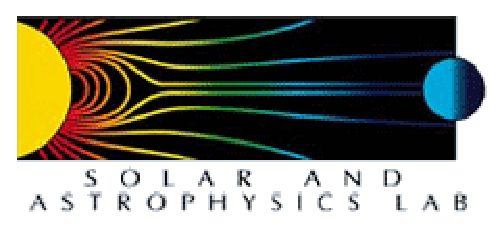
\includegraphics[height=0.1\linewidth]{logo_LMSAL.eps}}
\framebox{
\includegraphics[height=0.15\linewidth]{new_figs/logo_clasp2.eps}}
\salto
{\bf Binational AAA-SOCHIAS \textbar \ October-2018 \textbar \ La Serena, Chile}
\end{center}
  }

\begin{document}

%Pagina Inicial
\frame{\titlepage}

%-------------------> INTRODUCCION <----------------------------------------------------

\frame{
\titulo{Solar Corona and Sun-Earth relation}
\scriptsize
\framebox{\includegraphics[width=\linewidth]{new_figs/Sun-Earth.eps}}
\begin{center}
%La observación y el modelado de la Corona solar resulta de gran relevancia para el entendimiento de la relación Sol-Tierra, ya que en la Corona es donde el viento solar es calentado, acelerado y tienen lugar eventos impulsivos como eyecciones de masa coronal, flares, etc.

Being the place where the solar wind is heated and accelerated, and impulsive events as solar flares and coronal mass ejections are released, observation and modeling of the Solar Corona is of great relevance to advance our understanding of the Sun-Earth environment.
\end{center}
}

%-------------------------------------------------------------------
\begin{comment}
\frame{
\titulo{Solar Structure}
\scriptsize
\begin{columns}
\column{0.5\textwidth}
%\ \hskip 1cm \azul{Interior}
%\begin{itemize}
%\item Core (T$\approx 15$\, MK)
%\item Radiative Z. (T$\approx 10-0.5$\, MK)
%\item Convective Z. (T$\approx 0.5\,{\rm MK} - 6.5$\, kK)
%\end{itemize}
\vspace{0.55cm}
\begin{center}
{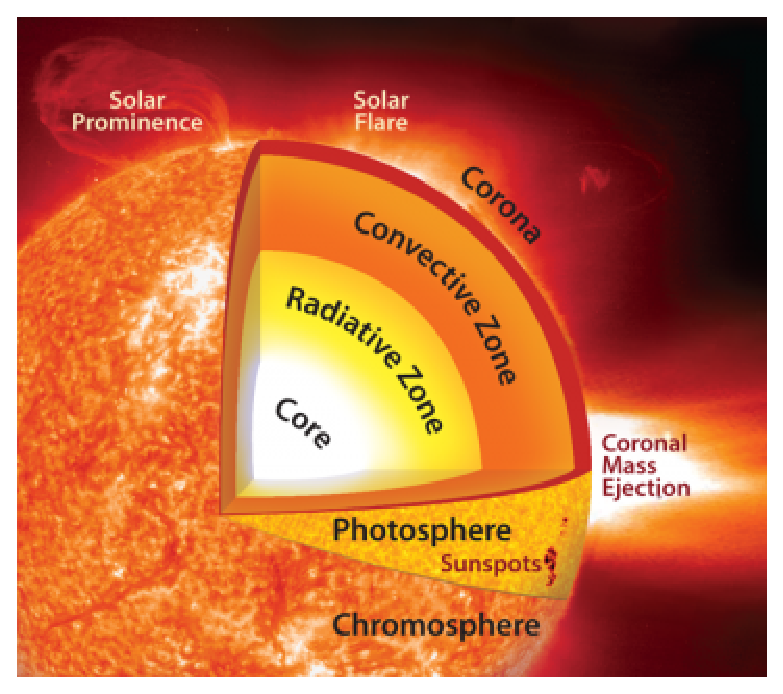
\includegraphics[width=0.9\textwidth]{new_figs/SolarStructure.eps}}
\end{center}
\column{0.55\textwidth}
\ \hskip 1cm \azul{Atmosphere}
\begin{itemize}
\item Photosphere (T $\approx 5.5$\, kK, $n \approx 10^{17}\ {\rm cm}^{-3}$)
\item Chromosphere (T $\approx 20$\, kK, $n \approx 10^{11}\ {\rm cm}^{-3}$)
\item Transition Region (Thickness 100 km)
\item Corona (T $\approx 1-10$\, MK, $n \approx 10^{10-7}\ {\rm cm}^{-3}$)
\end{itemize}
\begin{center}
{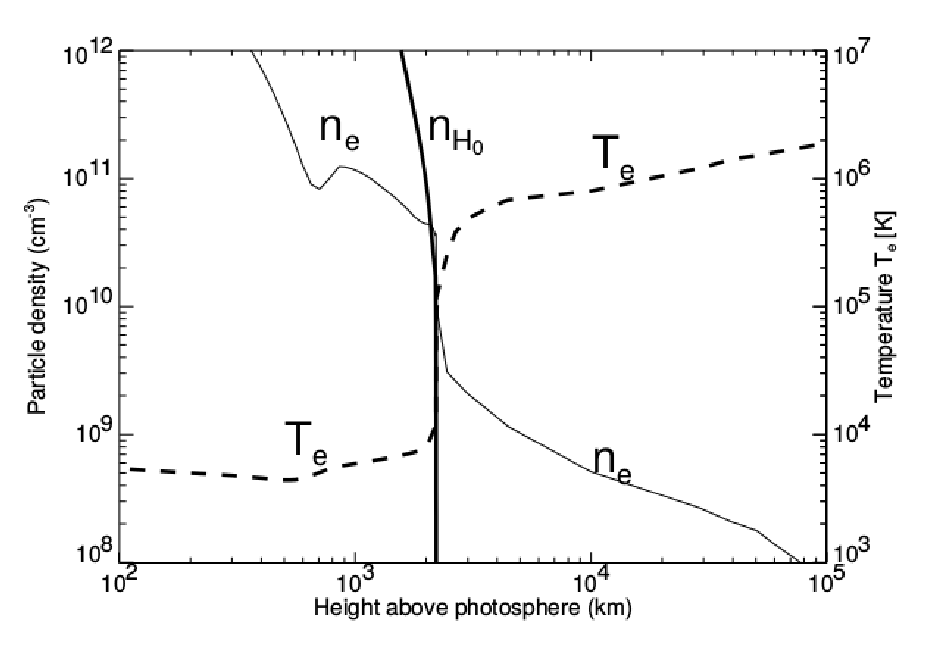
\includegraphics[width=0.675\textheight]{new_figs/region_transicion_fede.eps}}
\end{center}
\end{columns}
}
\end{comment}
%---------------------------------------------------------------------------
\frame{
\titulo{Solar Corona}
\footnotesize
\vspace{-0.25cm}
\begin{center}
{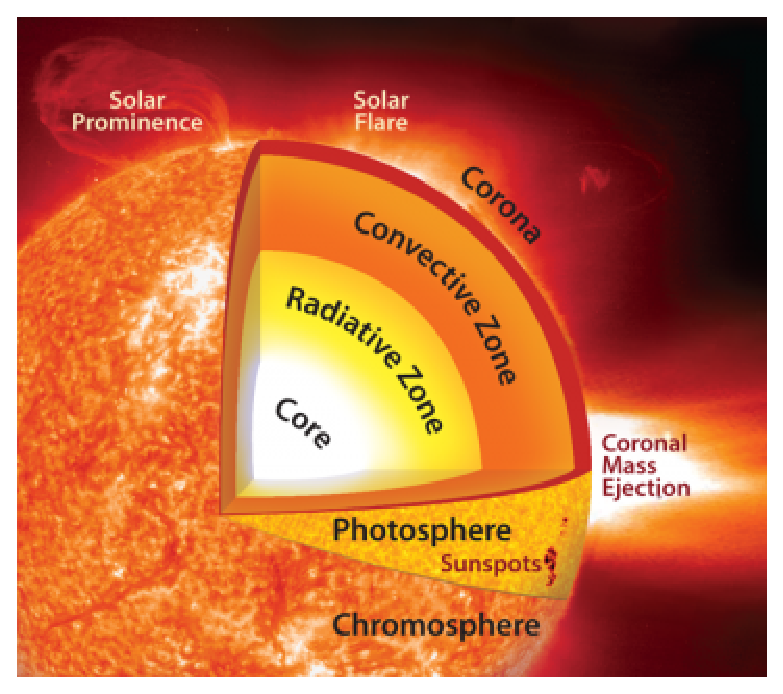
\includegraphics[width=0.35\textwidth]{new_figs/SolarStructure.eps}}
{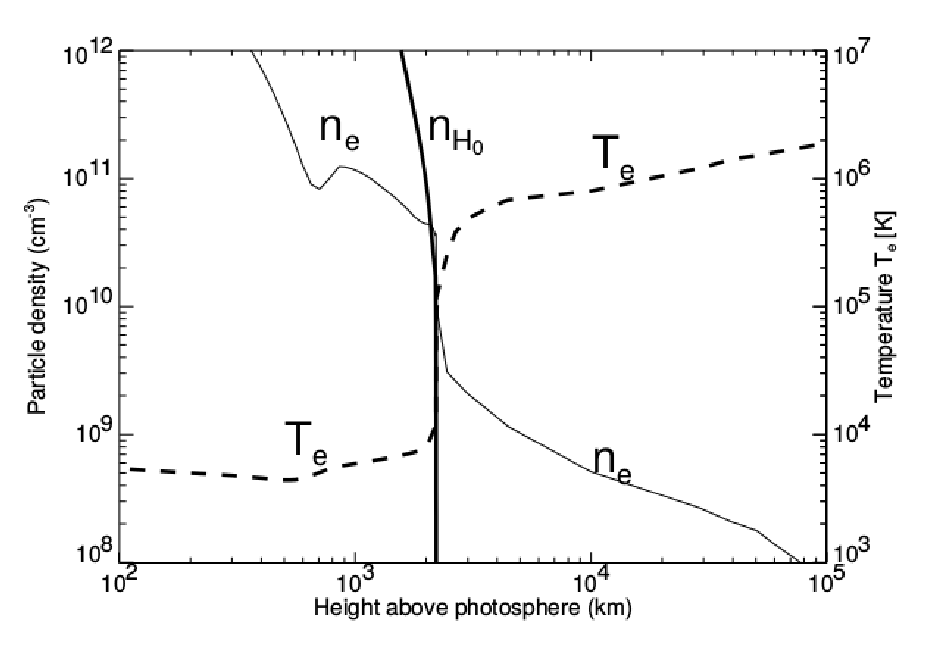
\includegraphics[width=0.45\textwidth]{new_figs/region_transicion_fede.eps}}
\end{center}
 Corona (T $\approx 1-10$\, MK, $n \approx 10^{10-7}\ {\rm cm}^{-3}$)
\begin{itemize}
 %\item La baja corona emite eficientemente en el rango EUV.\\
 \item The corona is \azul{optically thin} in the UV, \azul{EUV}, X, \azul{WL} ranges.\\
%Las imágenes son proyecciones 2D de estructuras emisoras 3D.
\item Images are thus 2D projections of the underlying 3D emitting structure.
% \salto
% \item El plasma emisor es governado por el \azul{campo magn\'etico coronal} congelado a la materia, para el cual {no se dispone de mediciones} (que son fotosf\'ericas).
 \mediosalto
%\item Los modelos físicos necesitan información 3D coronal de parámetros $N_e, T_e$.
\item Advancement of physical models is in need of 3D information of the coronal fundamental parameters ${\bf B}, N_e, T_e$ and chemical abundances.
\end{itemize}
\vspace{0.35cm}
\azul{\bf Tomography}\\
\vspace{0.15cm}
By inverting for the \azul{3D EUV emissivity from time series of images} it allows inferring the 3D $N_e$ and $T_e$ of the global corona.
%\begin{columns}
%\column{0.5\textwidth}
%\begin{center}
%AIA \\
%{\includegraphics[height=0.3\textwidth]{new_figs/2017_12_15_19_11_15_AIA_171.png}}
%{\includegraphics[height=0.3\textwidth]{new_figs/2017_12_15_19_11_15_AIA_193.png}}
%{\includegraphics[height=0.3\textwidth]{new_figs/2017_12_15_19_11_15_AIA_211.png}}
%\azul{\bf Stereoscopy}
%{\includegraphics[height=0.65\textwidth]{figuras/aia_171_loops.eps}}
%\\
%By studying the \azul{2D shape of EUV loops from 2 view points} it infers the 3D geometry of their "frozen-in" magnetic loops.
%\end{center}
%\column{0.5\textwidth}
%\begin{center}
%COSMO K-coronograph
%{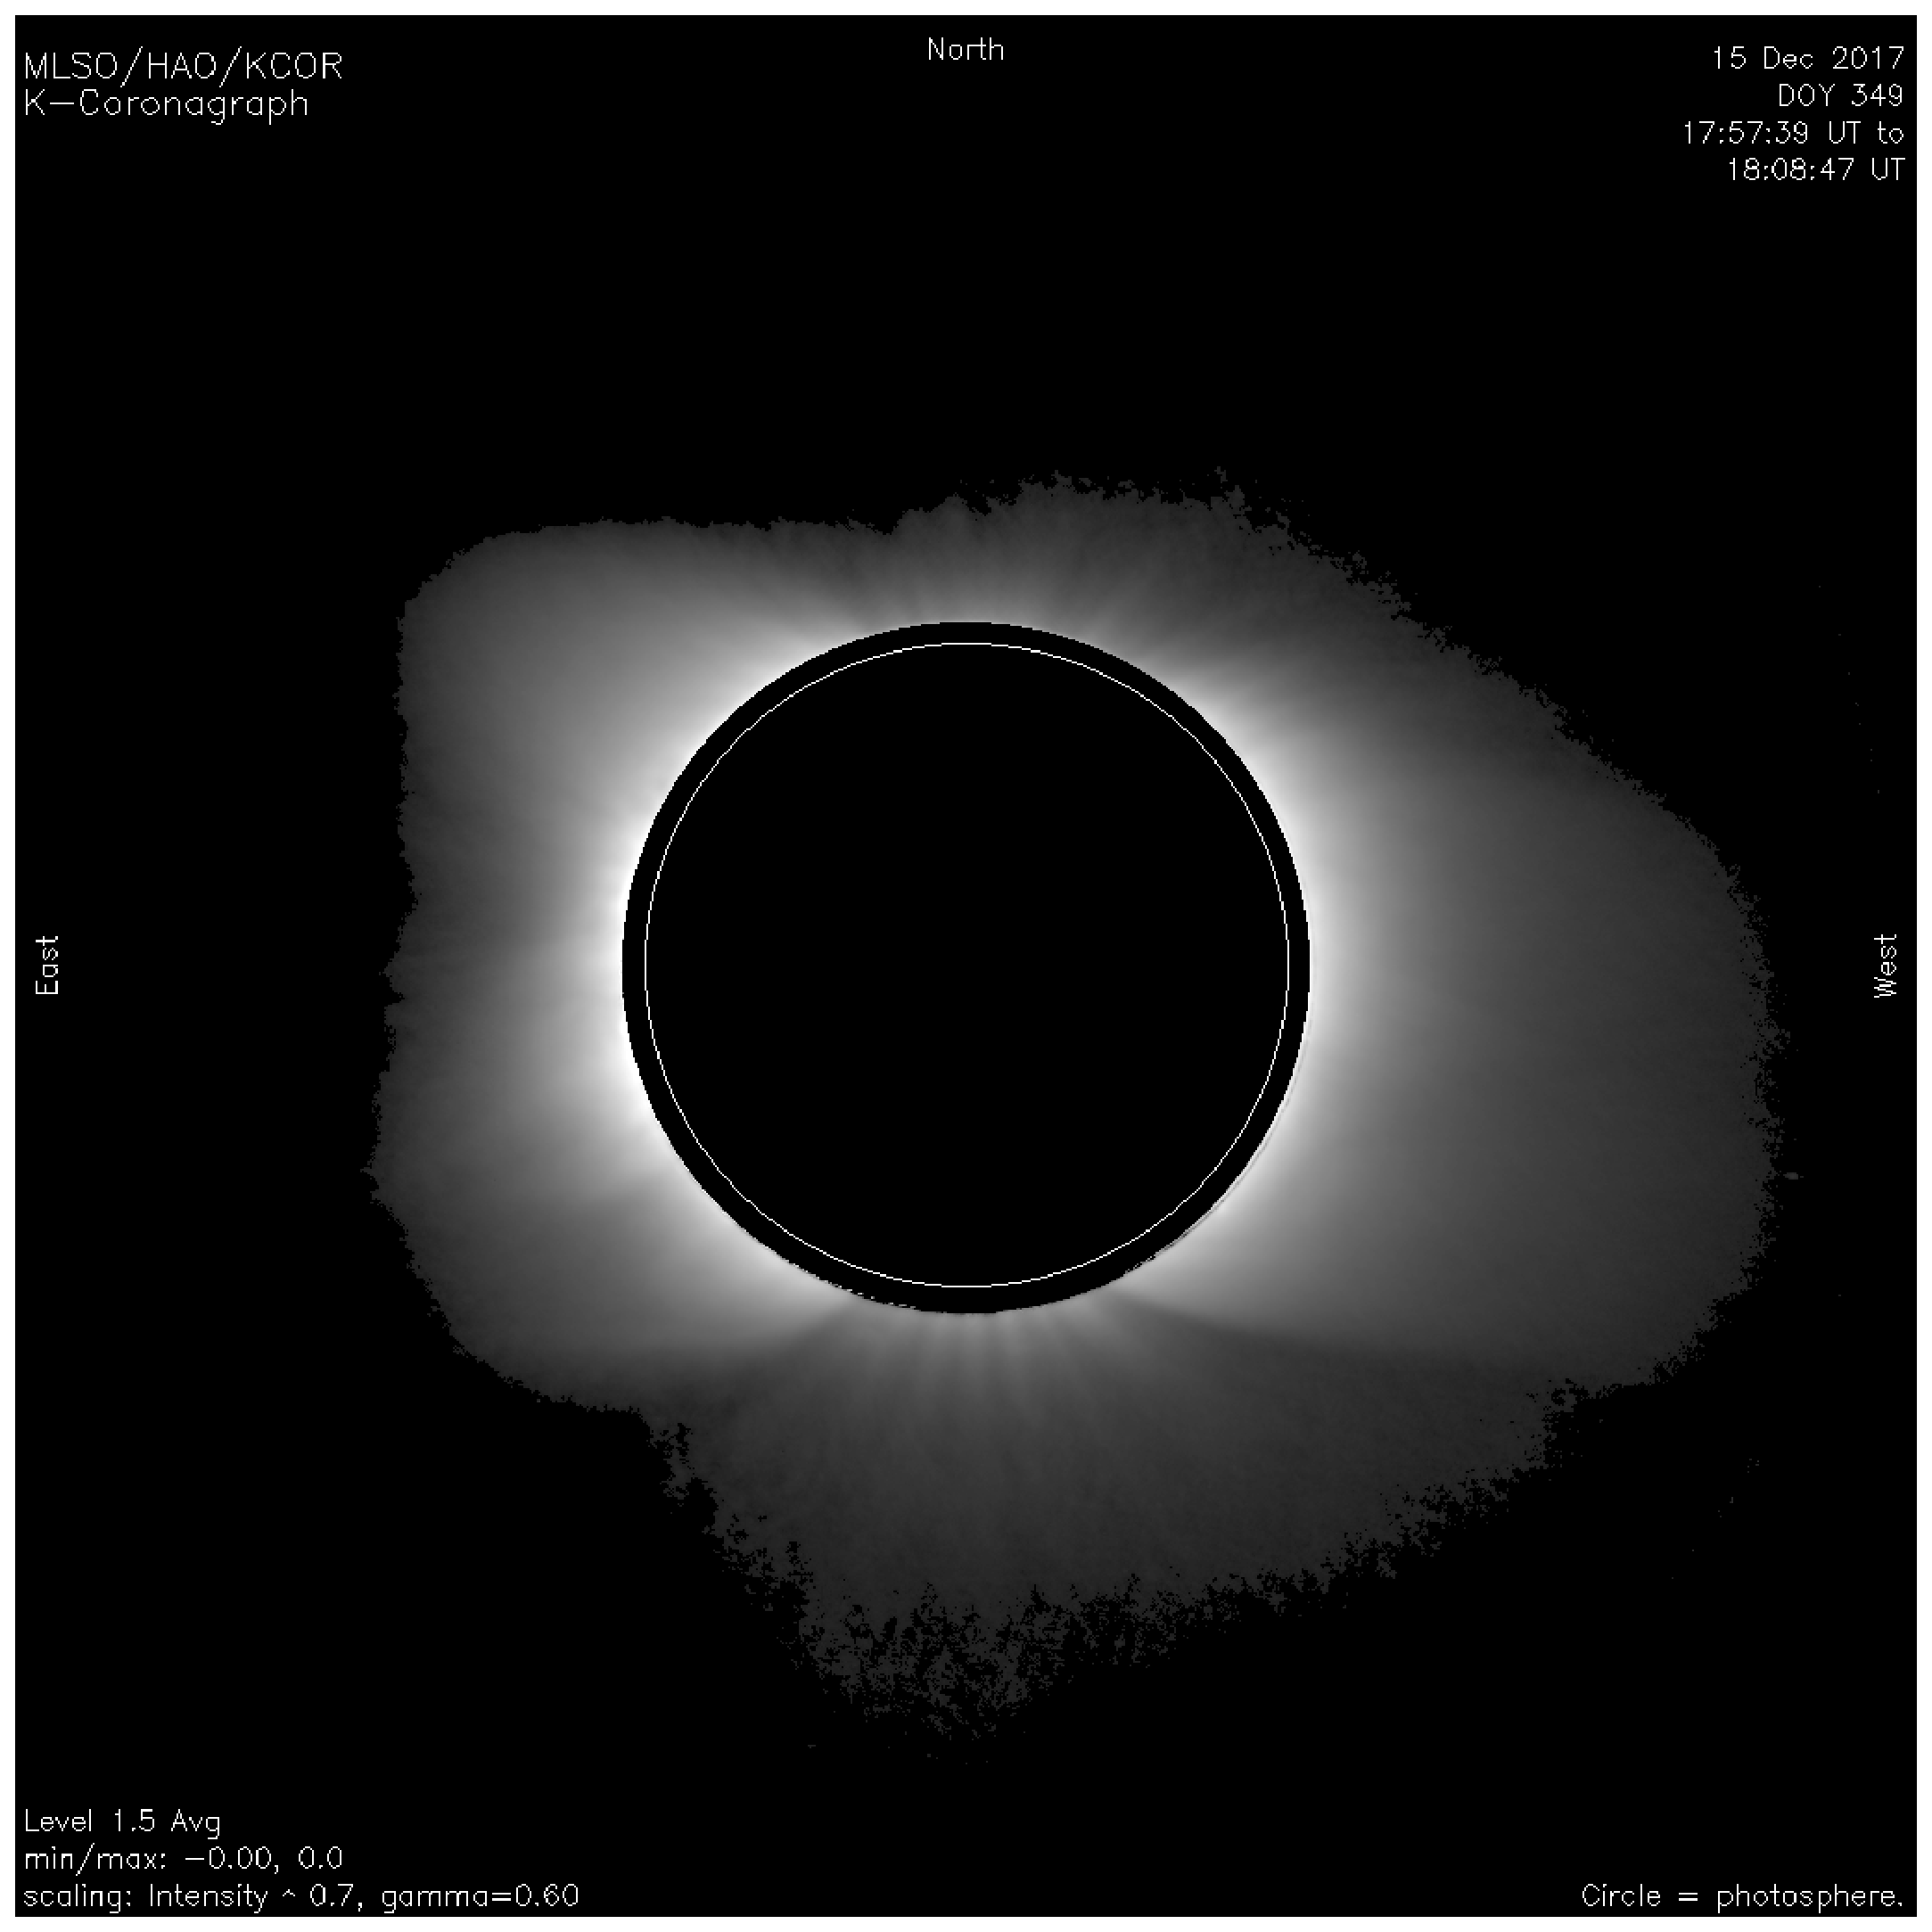
\includegraphics[height=0.7\textwidth]{new_figs/20171215_175739_kcor_l15_extavg.eps}}
%{\includegraphics[height=0.7\textwidth]{figuras/aia_193_fullsun.eps}}
%Invierte una serie temporal de imágenes EUV permitiendo inferir la distribución 3D de $N_e$ y $T_e$ en la baja corona.\\
%(Frazin et al. 2005)
%By inverting for the \azul{3D EUV emissivity from time series of images} it allows inferring the 3D $N_e$ and $T_e$ of the global corona.
%\end{center}
%\end{columns}

}
%------------------------------
\frame{
\titulo{Solar Rotational Tomography (SRT)}
\footnotesize
\vspace{-0.2cm}
\begin{center}
The object of study is the solar corona.\\
The solar rotation provides the necessary 360\deg view angles.
\end{center}
%\vspace{-1.5cm}
\begin{columns}
%\vspace{-1cm}
\column{0.6\textwidth}
\begin{itemize}
\item 
\azul{Corona-K:} Thomson scattering of photospheric  \azul{white light (WL)}. Data gathered with WL coronagraphs.
\item \azul{SRT-WL} $\rightarrow$ 3D $N_e$.
\item 1st SRT-WL: Altschuler \& Perry (1972)
\end{itemize}
\vskip 1cm
\begin{itemize}
\item \azul{Corona-E:} True coronal emission by ions UV, \azul{EUV} y X.
\item \azul{SRT-EUV} $\rightarrow$ 3D EUV emissivity  $\rightarrow$\\
3D $N_e$ y $T_e$
\item 1st SRT-EUV: Frazin et al. (2009)
\end{itemize}
\column{0.4\textwidth}
%\vskip 1.2cm
\begin{center}
\azul{White Light}
%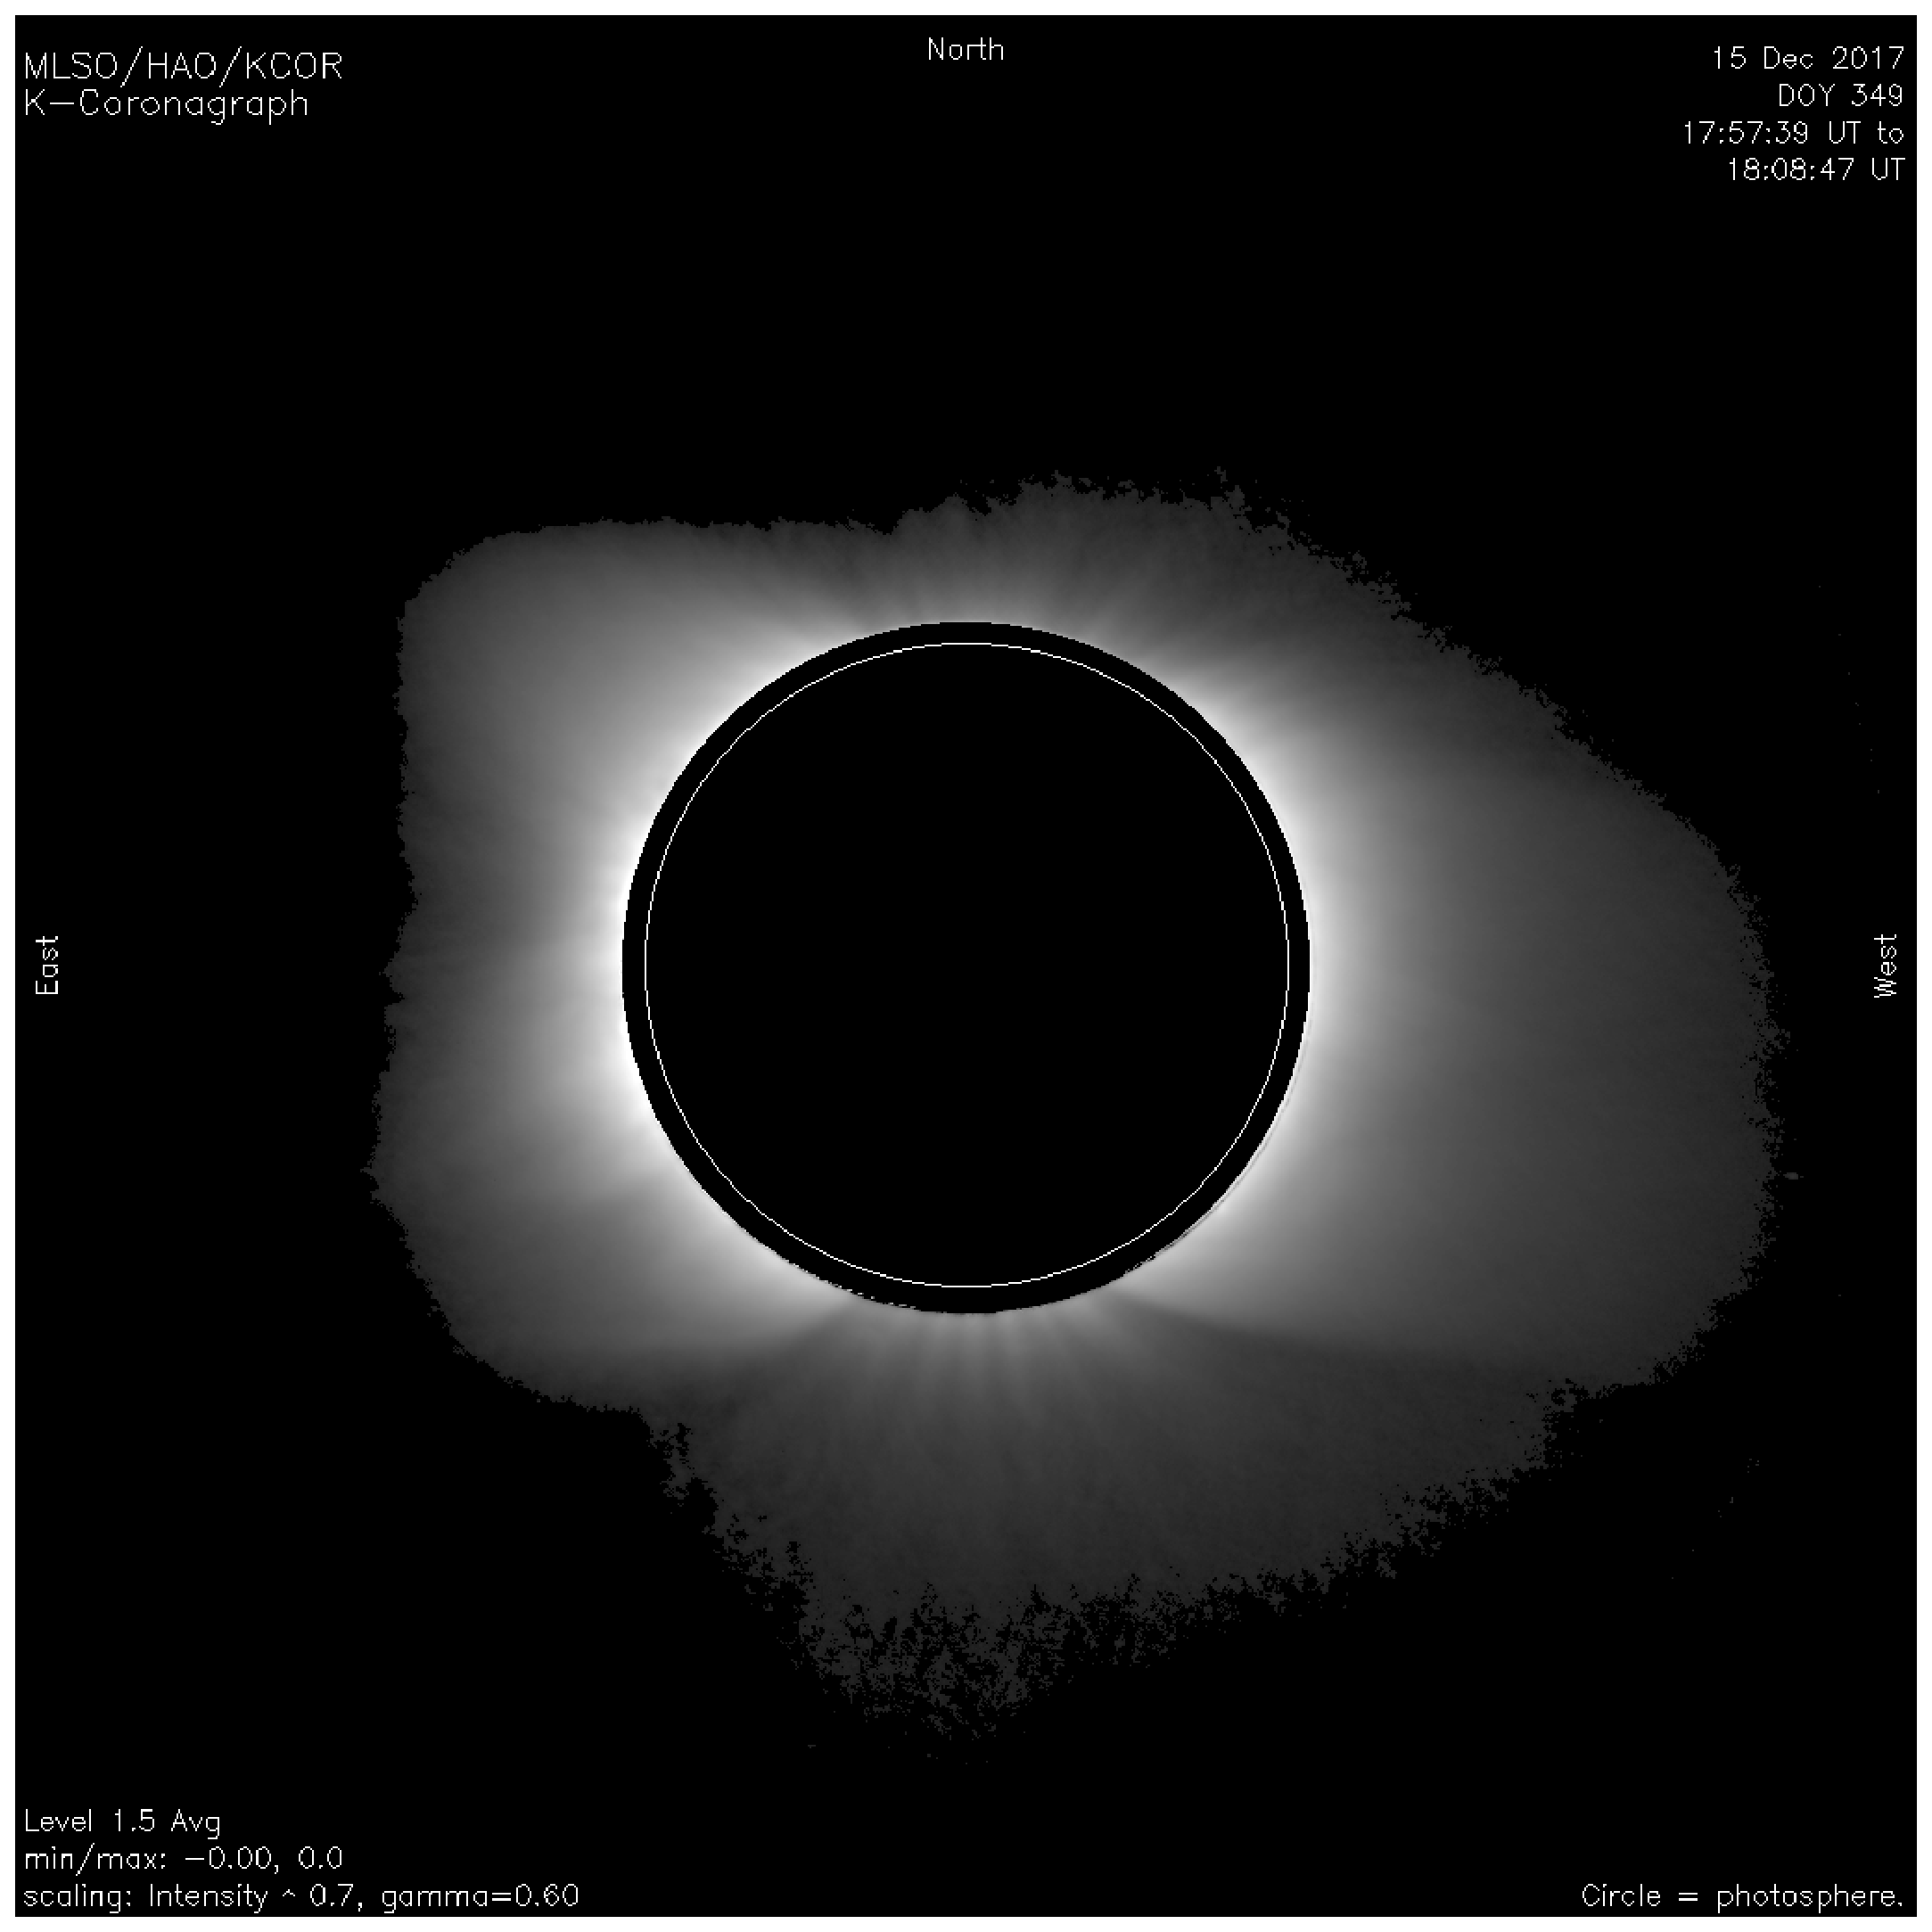
\includegraphics[height=0.7\textwidth]{new_figs/20171215_175739_kcor_l15_extavg.eps}
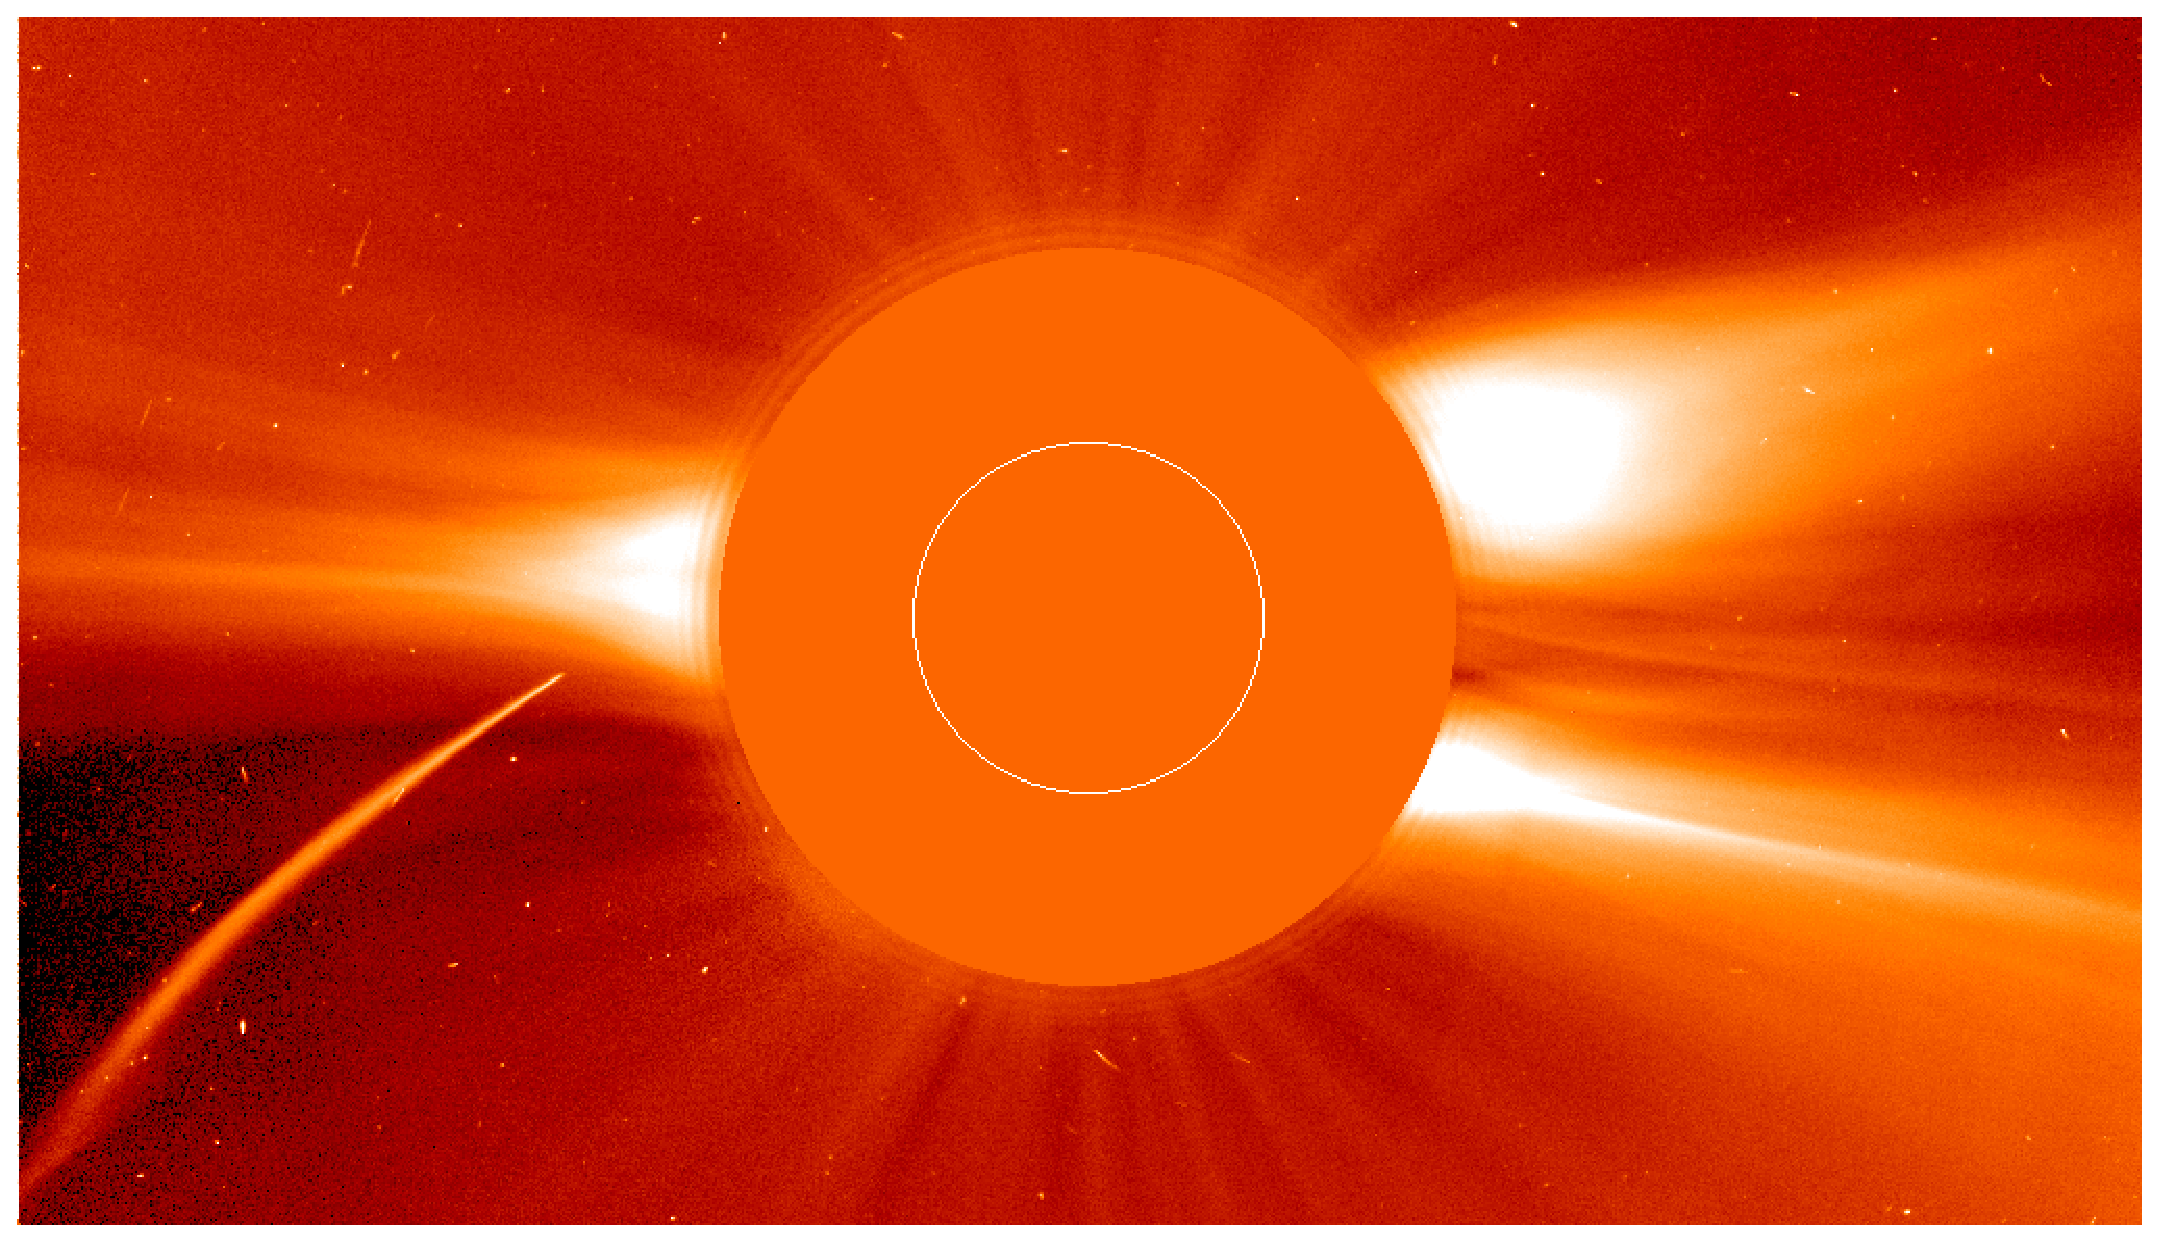
\includegraphics[height=0.6\textwidth]{new_figs/LASCOC2_comet.eps}
\mediosalto
\azul{EUV} \\
\includegraphics[height=0.6\textwidth]{new_figs/2017_12_15_19_11_15_AIA_171.png}
%\includegraphics[height=0.3\textwidth]{new_figs/2017_12_15_19_11_15_AIA_193.png}
%\includegraphics[height=0.3\textwidth]{new_figs/2017_12_15_19_11_15_AIA_211.png}
\end{center}
\end{columns}
}
%--------------------------------------
{
\setbeamercolor{normal text}{fg=white}
\setbeamercolor{frametitle}{fg=white}
\usebeamercolor[fg]{normal text}
\usebackgroundtemplate{\includegraphics[width=\paperwidth]{new_figs/orbits.eps}}
\frame{
\titulo{Full-Sun EUV Space Telescopes}
\scriptsize
\vspace{-1.75cm}
\begin{center}
%\begin{itemize}
%\item
Extreme ultraviolet Imaging Telescope {\bf (EIT)}\\ 
Solar and Heliospheric Observatory {\bf(SOHO)}\\
1996-2005. Sun-Earth L1 orbit.
%\salto
%\item
%Transition Region And Coronal Explorer \azul{(TRACE)}. 1998-2010.\\
%Sun-synchronous low Earth orbit (LEO).
\salto
%\item
Extreme UltraViolet Imager {\bf (EUVI)}\\
Solar TErrestrial RElations Observatory {\bf(STEREO)}\\ 
2007-2023. Two 1AU orbits behind and ahead Earth.
\salto
%\item
%Atmospheric Imaging Assembly {\bf (AIA)}\\ 
%Solar Dynamics Observatory {\bf(SDO)}\\ 
%2010-2020. Geosynchronic orbit around Earth.
%\end{itemize}
\end{center}
\vspace{-0.5cm}
\begin{table}[ht]
%\begin{center}
\begin{tabular}{llll}
\hline
Instrument & EIT  & EUVI \\%& AIA\\
\hline
\# Coronal Bands & 3  & 3  \\%& 6\\
Temperature range (MK) & 
[0.5,3.0] & [0.5,3.0] \\%& [0.5,15]\\
F.O.V. (\rsun) & 2.8  & 3.4 \\% & 2.6 \\
%Image size & $1024^2$ & $2048^2$ & $4096^2$\\
%Resolution [arc sec; $10^{-3}$\rsun]  & 2.6 & 1.6 & 0.6\\
\hline
\end{tabular}
%\end{center}
\end{table}
}
}
%-----------------------------------
\frame{ 
\vspace{-0.35cm}
\begin{columns}
\noindent
\column{0.075\textwidth}
\vskip 0.8cm
{\footnotesize
\ 171 \AA
\vskip 1.75cm
\ 195 \AA
\vskip 1.65cm
\ 284 \AA
}
\column{\textwidth}
\begin{center}
{\footnotesize
\ \ Data Images \hfill $\rightarrow$ \hfill 3D Band Emissivity \hfill $\rightarrow$ \hfill Synthetic Images\ \ \ \
}\\
\framebox{\includegraphics[width=0.95\linewidth]{new_figs/frame_050_test.pdf}}\\
\footnotesize
 1.035 $\mrsun$ \hskip 1cm 1.085 $\mrsun$ \hskip 1cm 1.135 $\mrsun$ \hfil
\end{center}
\end{columns}
\begin{columns}
 \column{0.4\textwidth}
 Vásquez et al. (2016)
 \column{0.6\textwidth}
\end{columns}
}
%-------------------------------
\frame{
\titulo{Characteristic Temperatures of the Solar Corona}
\footnotesize
\begin{center}
EIT/SOHO and EUVI/STEREO \azul{3 bands:} \azul{0.5-2.75 MK}\\
{AIA/SDO} \azul{4 bands:} \azul{0.5-4.0 MK},\\
\begin{figure}[ht]
\figu{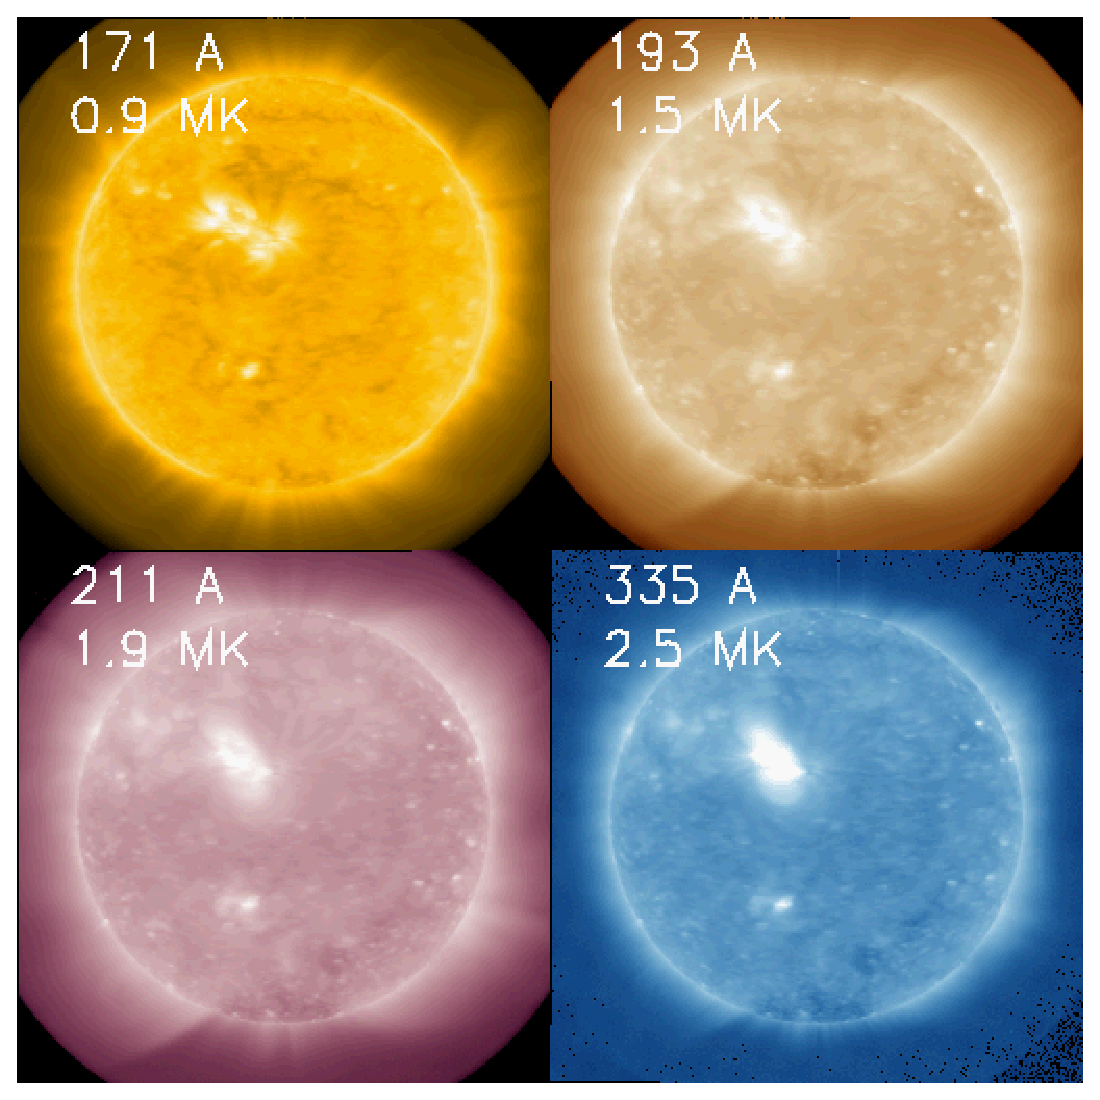
\includegraphics[height=0.375\linewidth]{new_figs/panel.eps}}
\figu{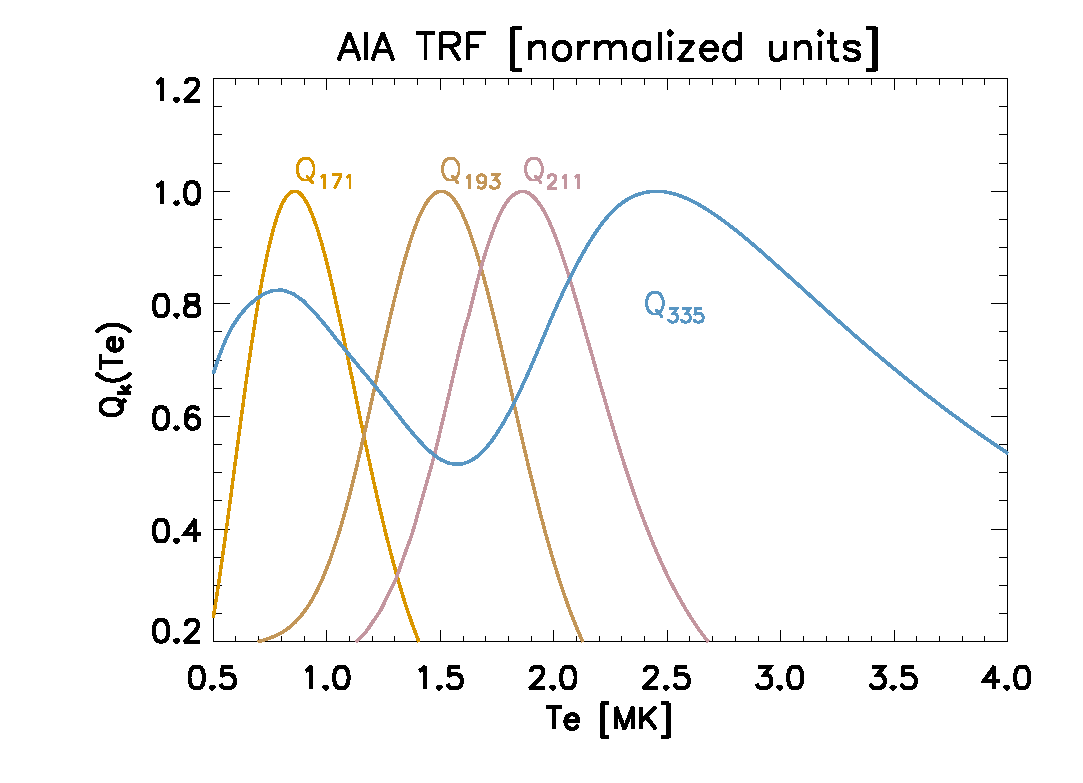
\includegraphics[height=0.375\linewidth]{new_figs/qkl.eps}}
\end{figure}
\end{center}
}

%---------------------------------
\frame{ 
\vspace{-0.05cm}
\titulo{Tomographic Results}
\footnotesize
\begin{columns}
\column{0.5\textwidth}
\hfil Minimum 2009 \\ Extreme UltraViolet Imager
{\includegraphics[width=0.86\textwidth]{new_figs/Ne_1105_cr2081l075_ldem_v3_errorbox_base_test.jpg}}
%\hskip 0.1cm
{\includegraphics[width=0.86\textwidth]{new_figs/Tm_1105_cr2081l075_ldem_v3_errorbox_base_test.jpg}}\\

\column{0.5\textwidth}
\hfil Minimum 1996 \\ Extreme ultraviolet Imaging Telescope
{\includegraphics[width=0.86\textwidth]{new_figs/Ne_1105_cr1915l075_ldem_v3_errorbox_base_test.jpg}}
%\hskip 0.1cm
{\includegraphics[width=0.86\textwidth]{new_figs/Tm_1105_cr1915l075_ldem_v3_errorbox_base_test.jpg}}\\
\end{columns}
(Lloveras et al. 2017)
}
%---------------------------------
\begin{comment}
\frame{
%\titulo{Instruments}
\footnotesize
\begin{columns}
\column{0.33\textwidth}
\begin{center}
Instruments \\
AIA - SDO\\
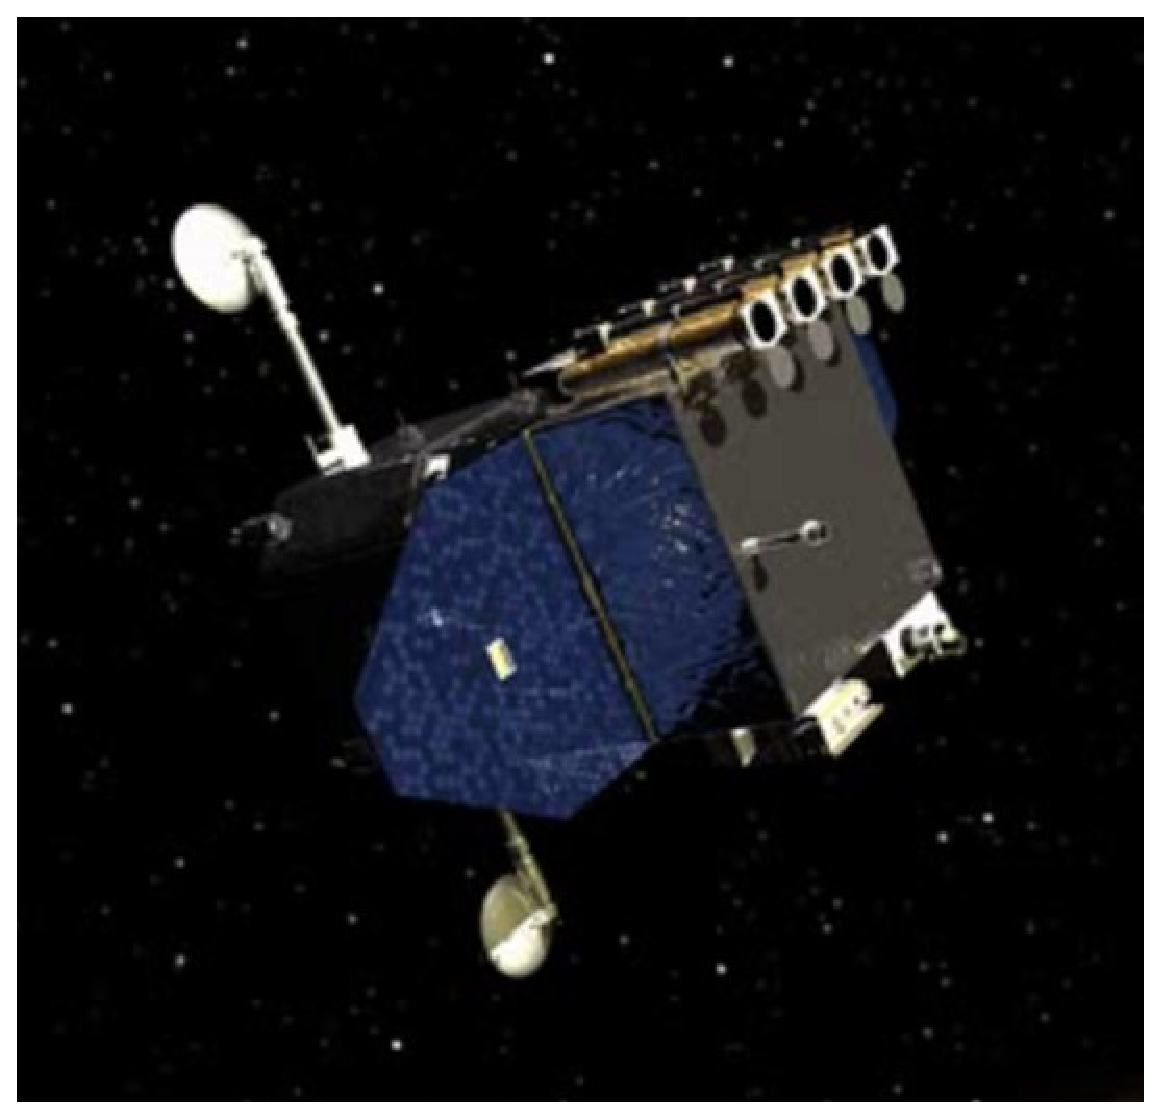
\includegraphics[height=0.6\textwidth]{new_figs/sdo.eps} \\
\mediosalto
K-Coronograph - COSMO \\
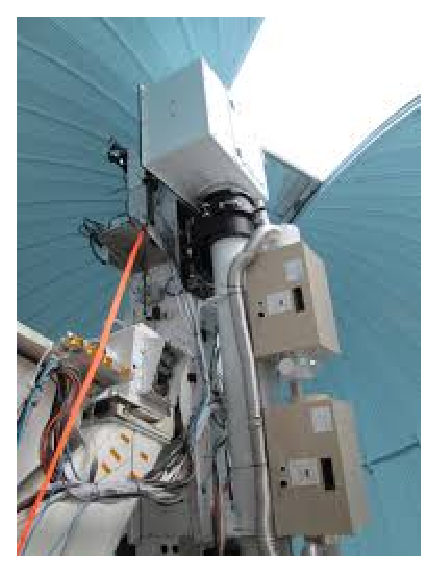
\includegraphics[height=0.9\textwidth]{new_figs/kcor.eps}
\end{center}
\column{0.33\textwidth}
\begin{center}
Images\\
Emission of the Fe lines \\
\includegraphics[height=0.33\textwidth]{new_figs/2017_12_15_19_11_15_AIA_171.png}
\includegraphics[height=0.33\textwidth]{new_figs/2017_12_15_19_11_15_AIA_193.png}
\includegraphics[height=0.33\textwidth]{new_figs/2017_12_15_19_11_15_AIA_211.png}
\mediosalto
\mediosalto
Polarized brightness \\
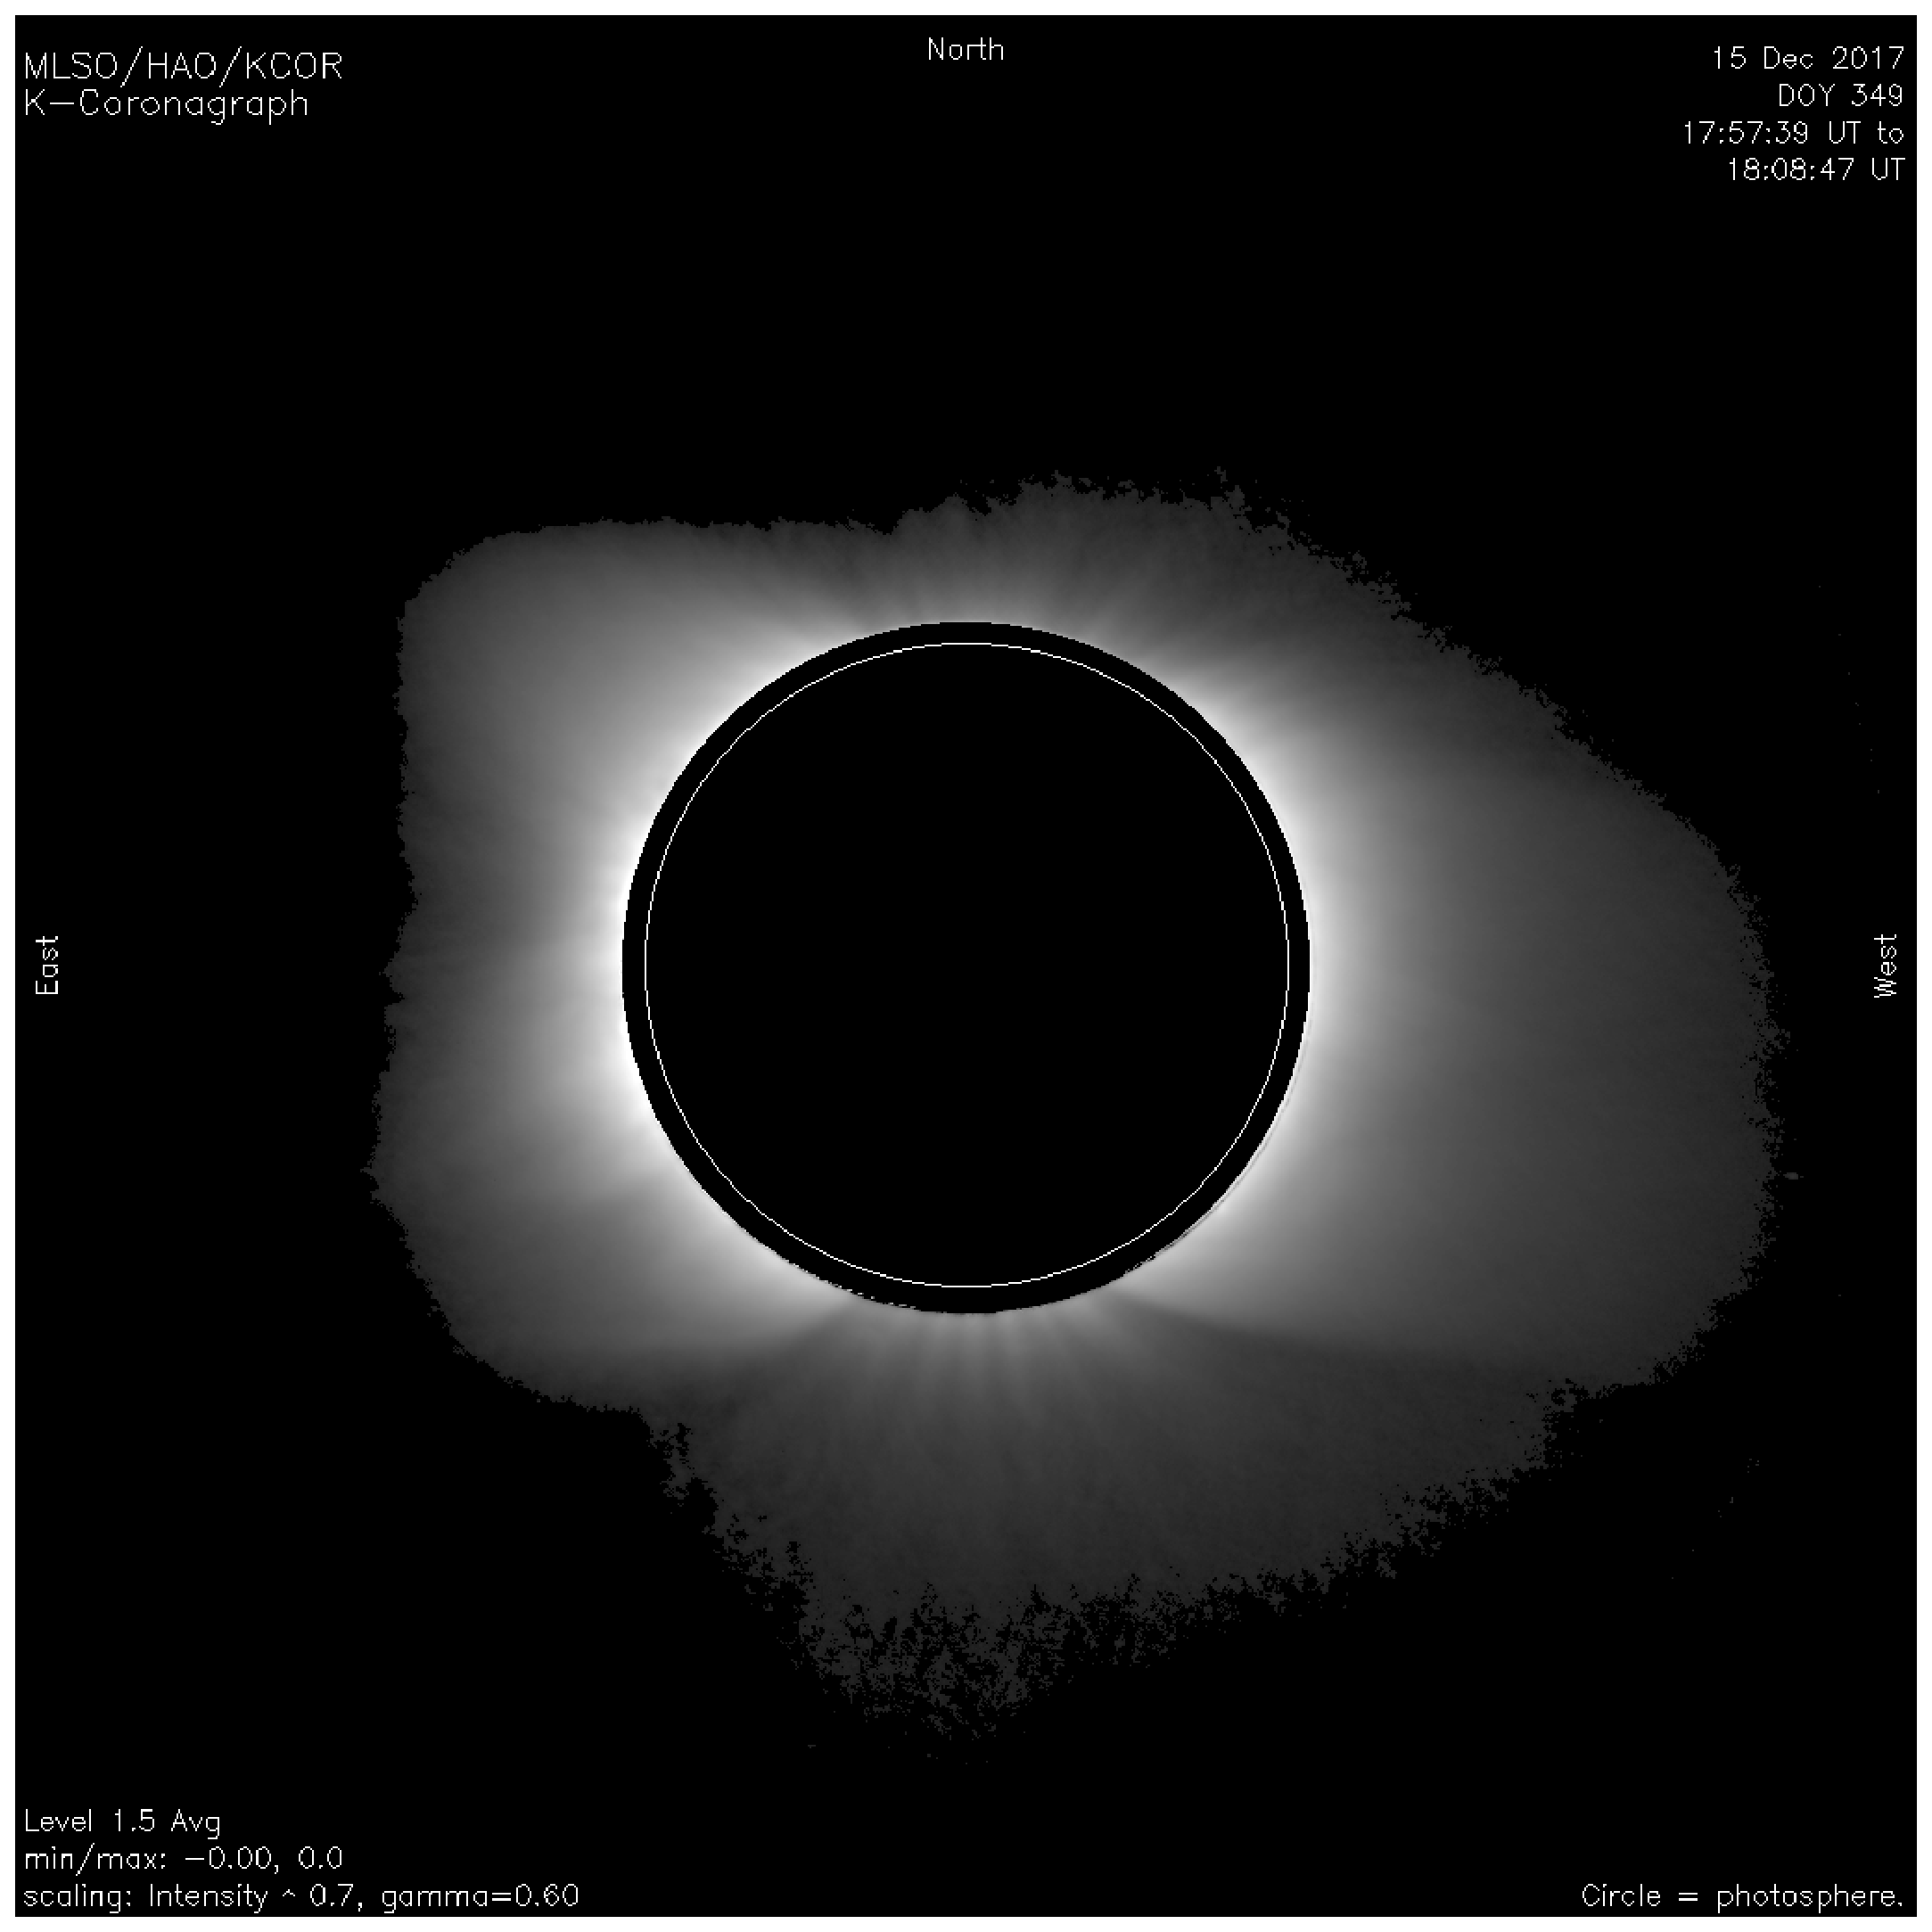
\includegraphics[height=0.9\textwidth]{new_figs/20171215_175739_kcor_l15_extavg.eps}
\end{center}
\column{0.33\textwidth}
\begin{center}
\vskip -1.6cm
$\rightarrow$ 3D $<{N_{e}}^{2}>$ \\
\vskip 2.cm
$\rightarrow$ 3D $<N_{e}>$
\end{center}
\end{columns}
}
\end{comment}
%----------------------------------
\frame{
\titulo{DEMT as MHD Validation Tool \azul{\footnotesize (Jin et al. 2012)}}
\footnotesize
\vspace{-0.25cm}
\begin{center}
2 Temp MHD Model of the Space Weather Modeling Framework (AOSS)
\vspace{-0.5cm}
\begin{columns}
\column{0.5\textwidth}
\begin{center}
\figu{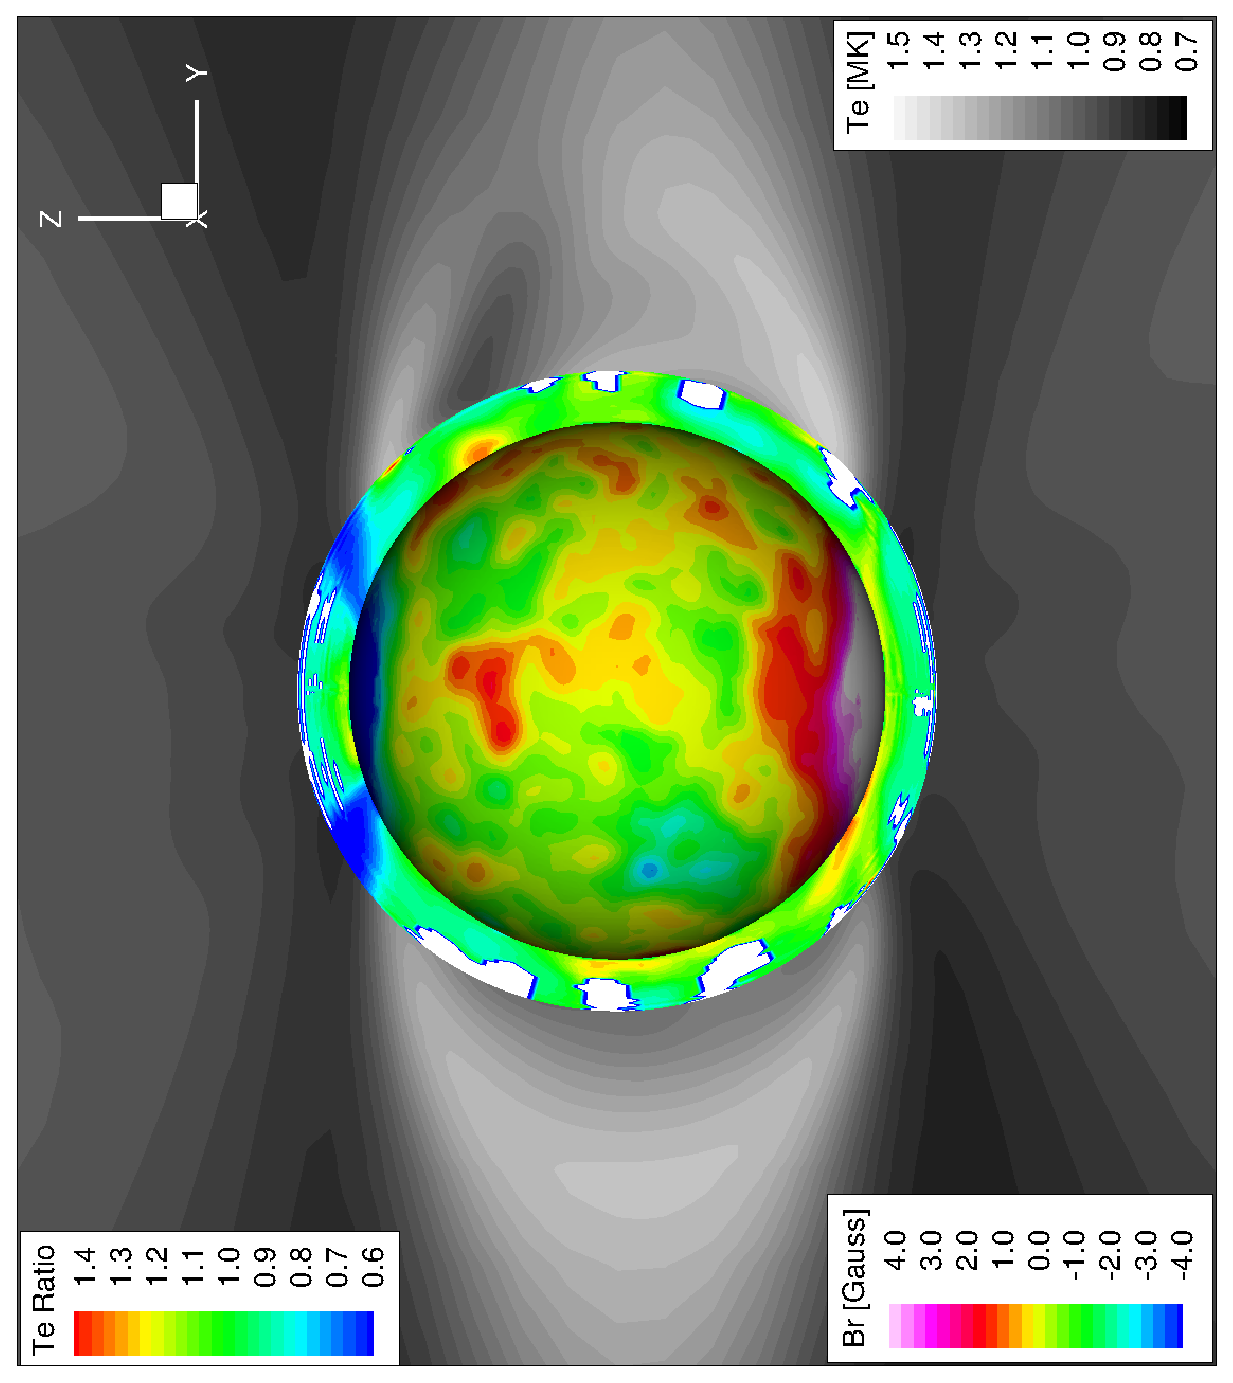
\includegraphics[width=0.85\textwidth,angle=-90]{new_figs/fig3_1.eps}}
\end{center}
\column{0.5\textwidth}
\begin{center}
\figu{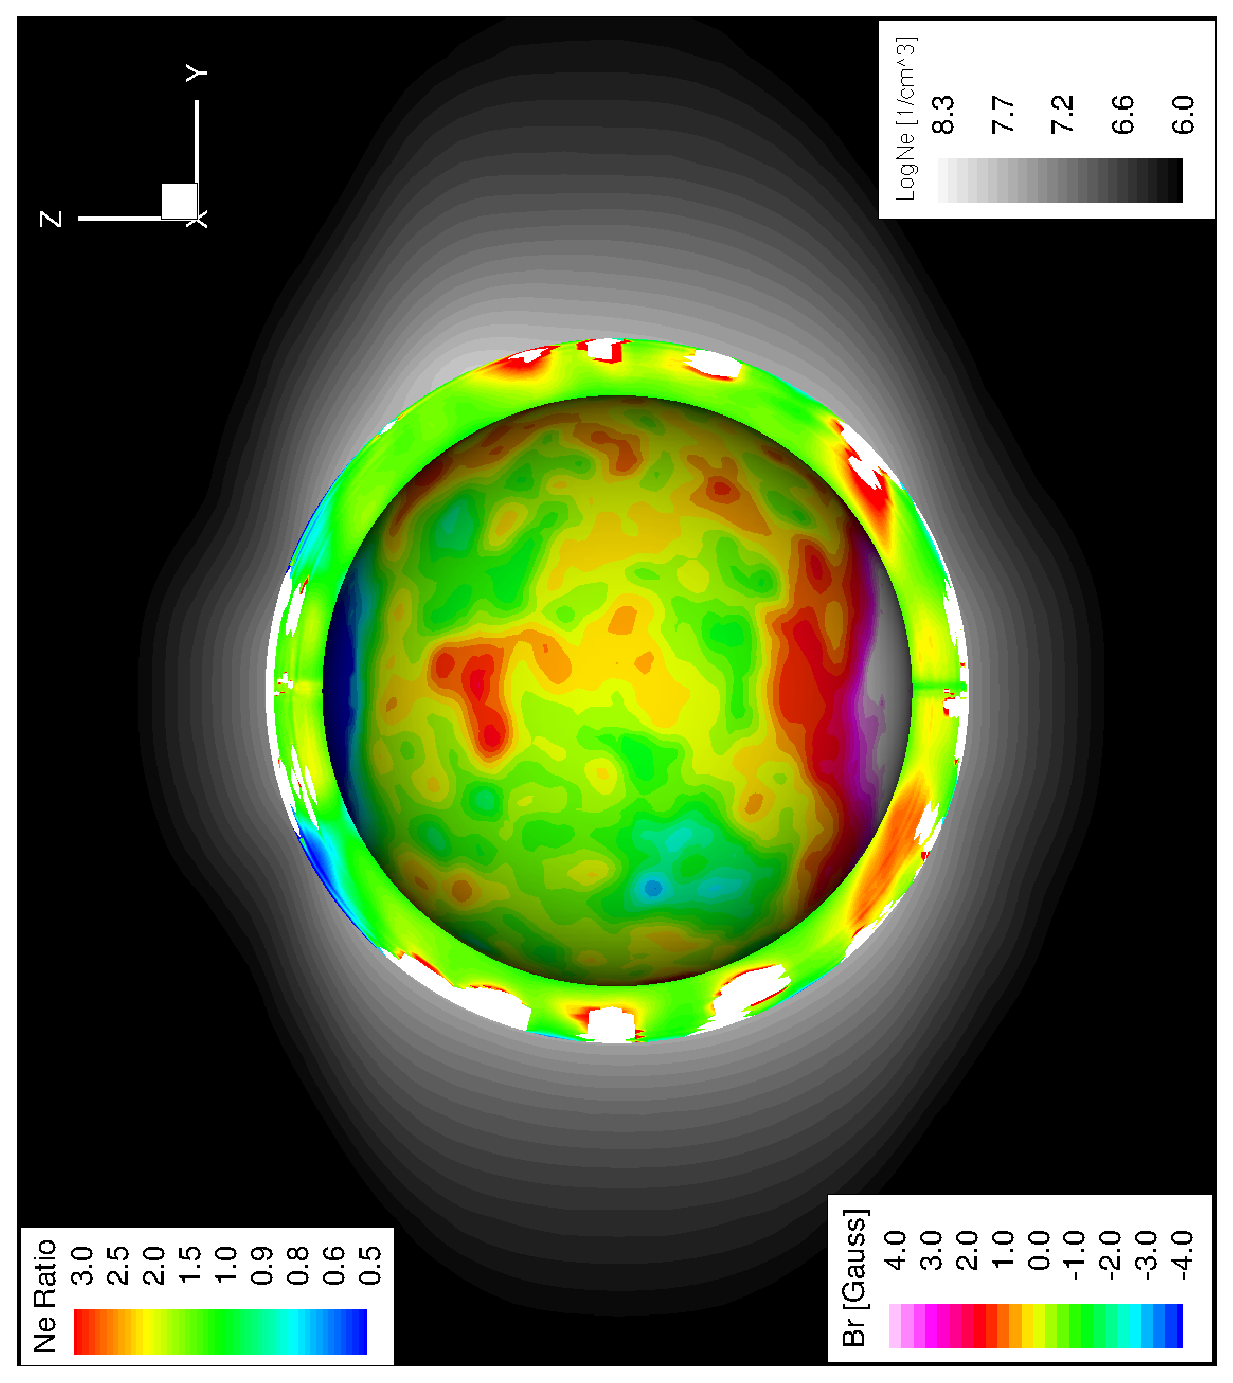
\includegraphics[width=0.85\textwidth,angle=-90]{new_figs/fig3_2.eps}}
\end{center}
\end{columns}
\end{center}
\begin{itemize}
\item
Inner Ring (1.00 - 1.25 \rsun): Ratio MHD/DEMT.\\
- Outter Greyscale map ($>$ 1.25 \rsun): MHD Model.\\
- Color Sphere: $B_r(1\,{\rm R_{\rm SUN}})$.
%\item
%$N_e$ y $T_e$ also validated with spectral analysis (Hinode/EIS, 1.02-1.10 \rsun).
\end{itemize}
}
%---------------------------------
\frame{
\titulo{EUV Ne Vs. WL Ne}
\vspace{-1.cm}
\footnotesize
\begin{center}
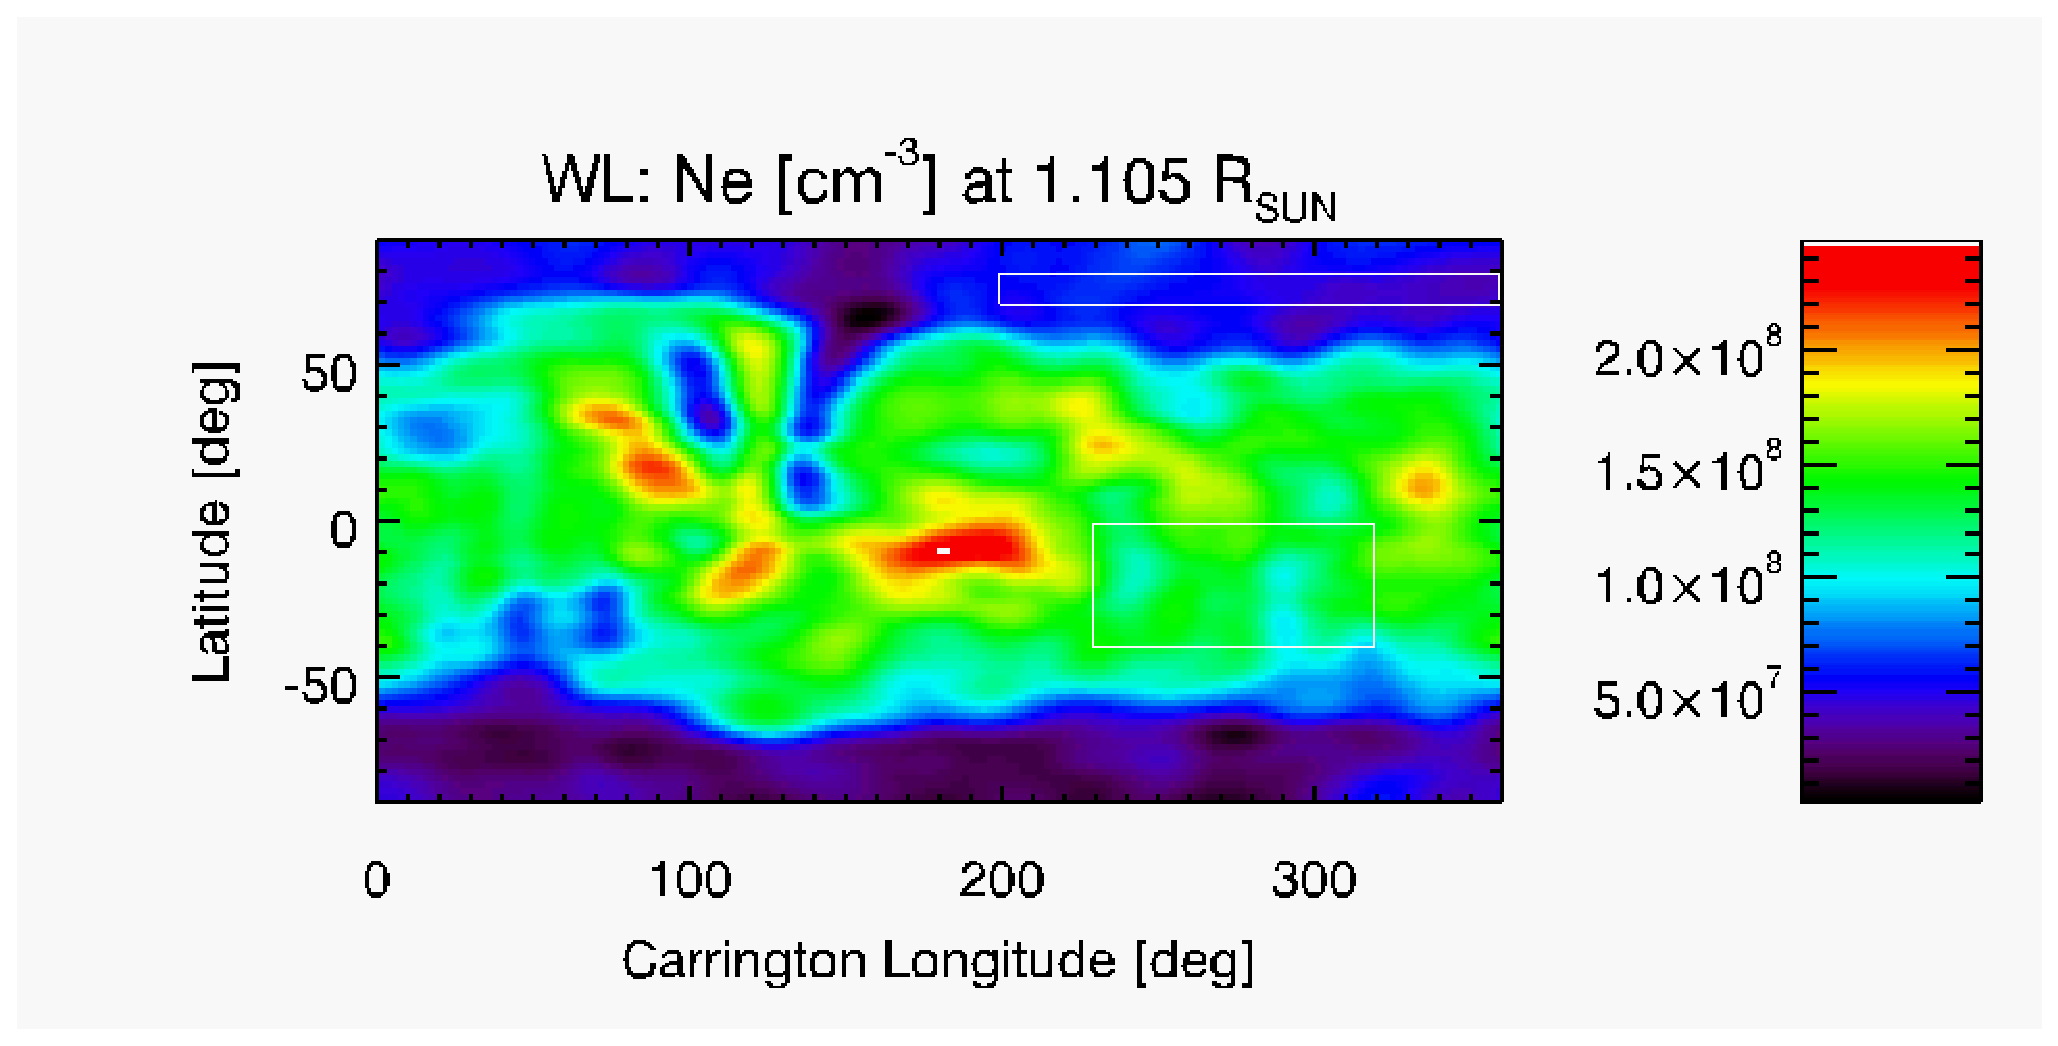
\includegraphics[height=0.5\textheight]{new_figs/map_ne_kcor.eps}\\ 
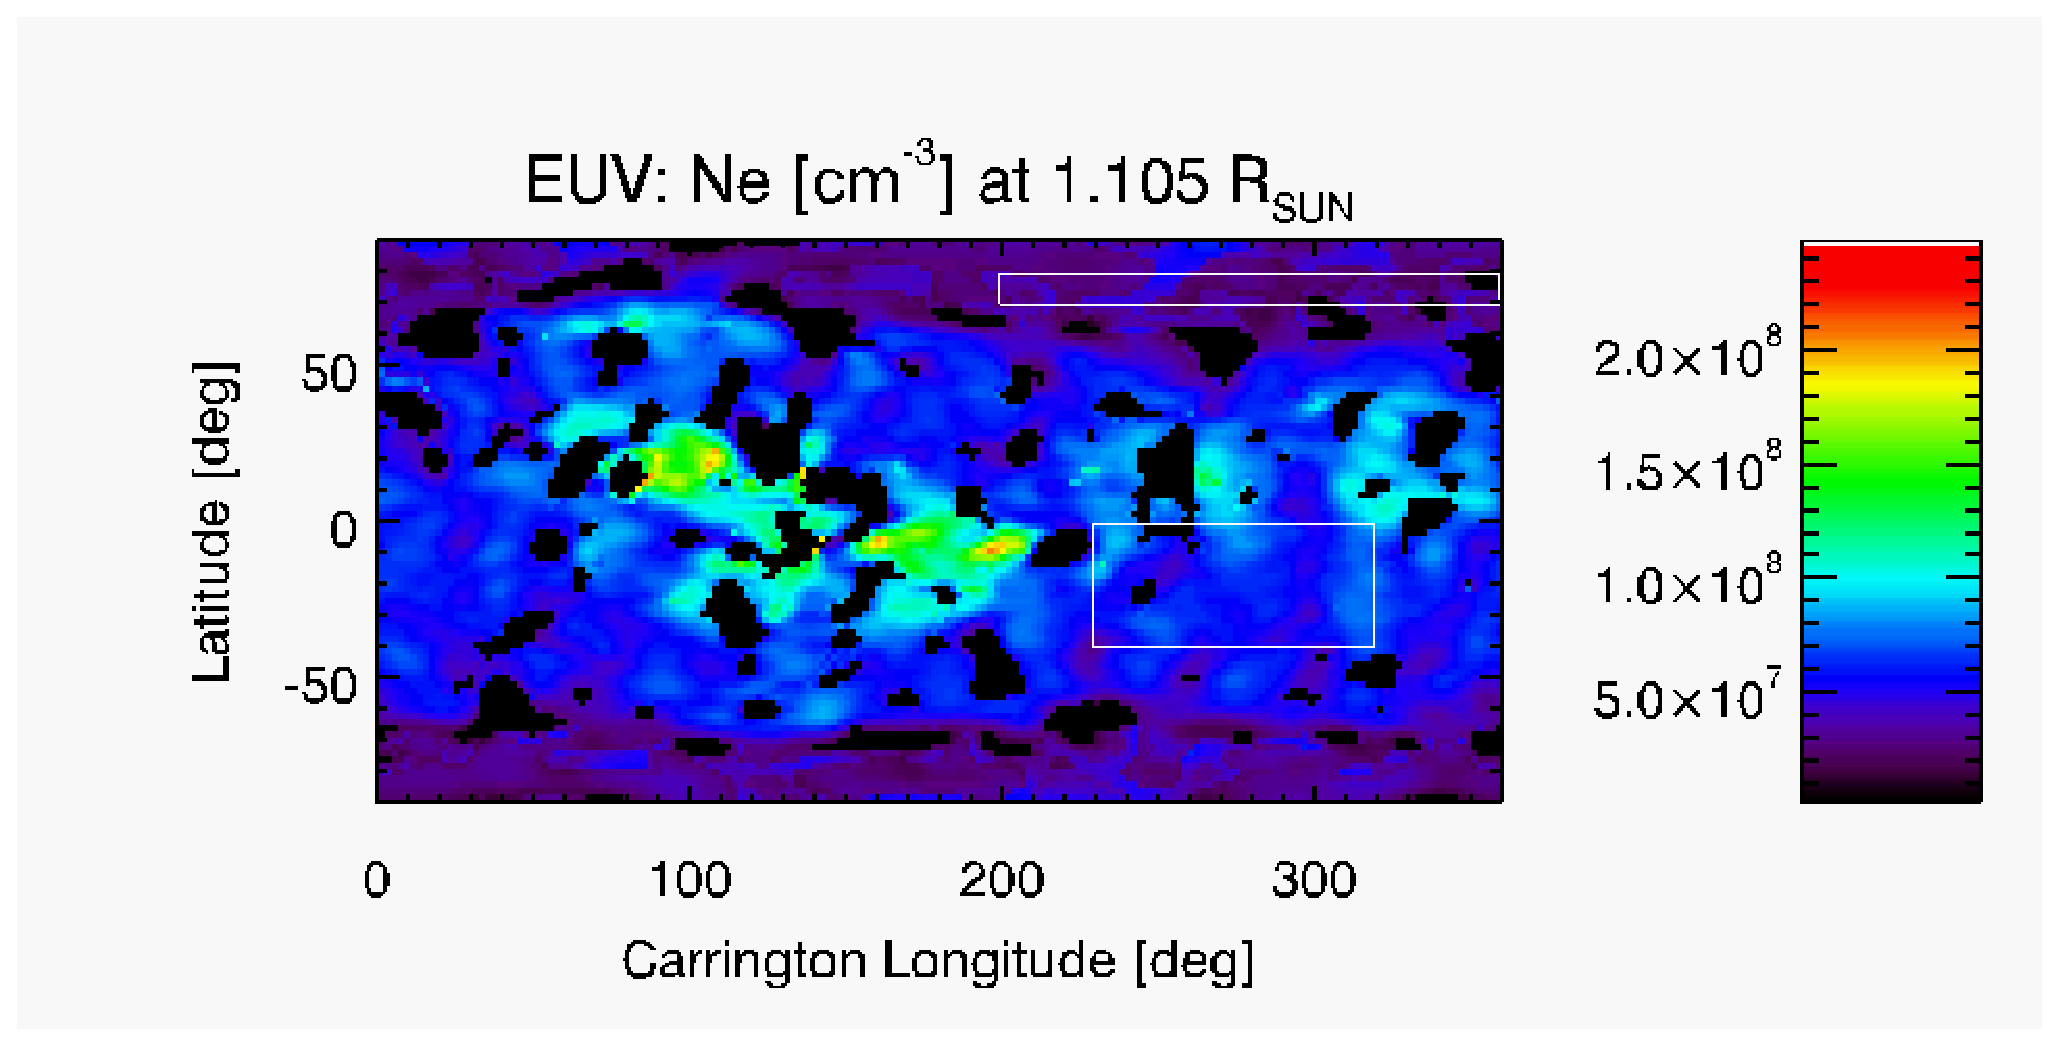
\includegraphics[height=0.5\textheight]{new_figs/map_ne_aia.eps}
\end{center}
%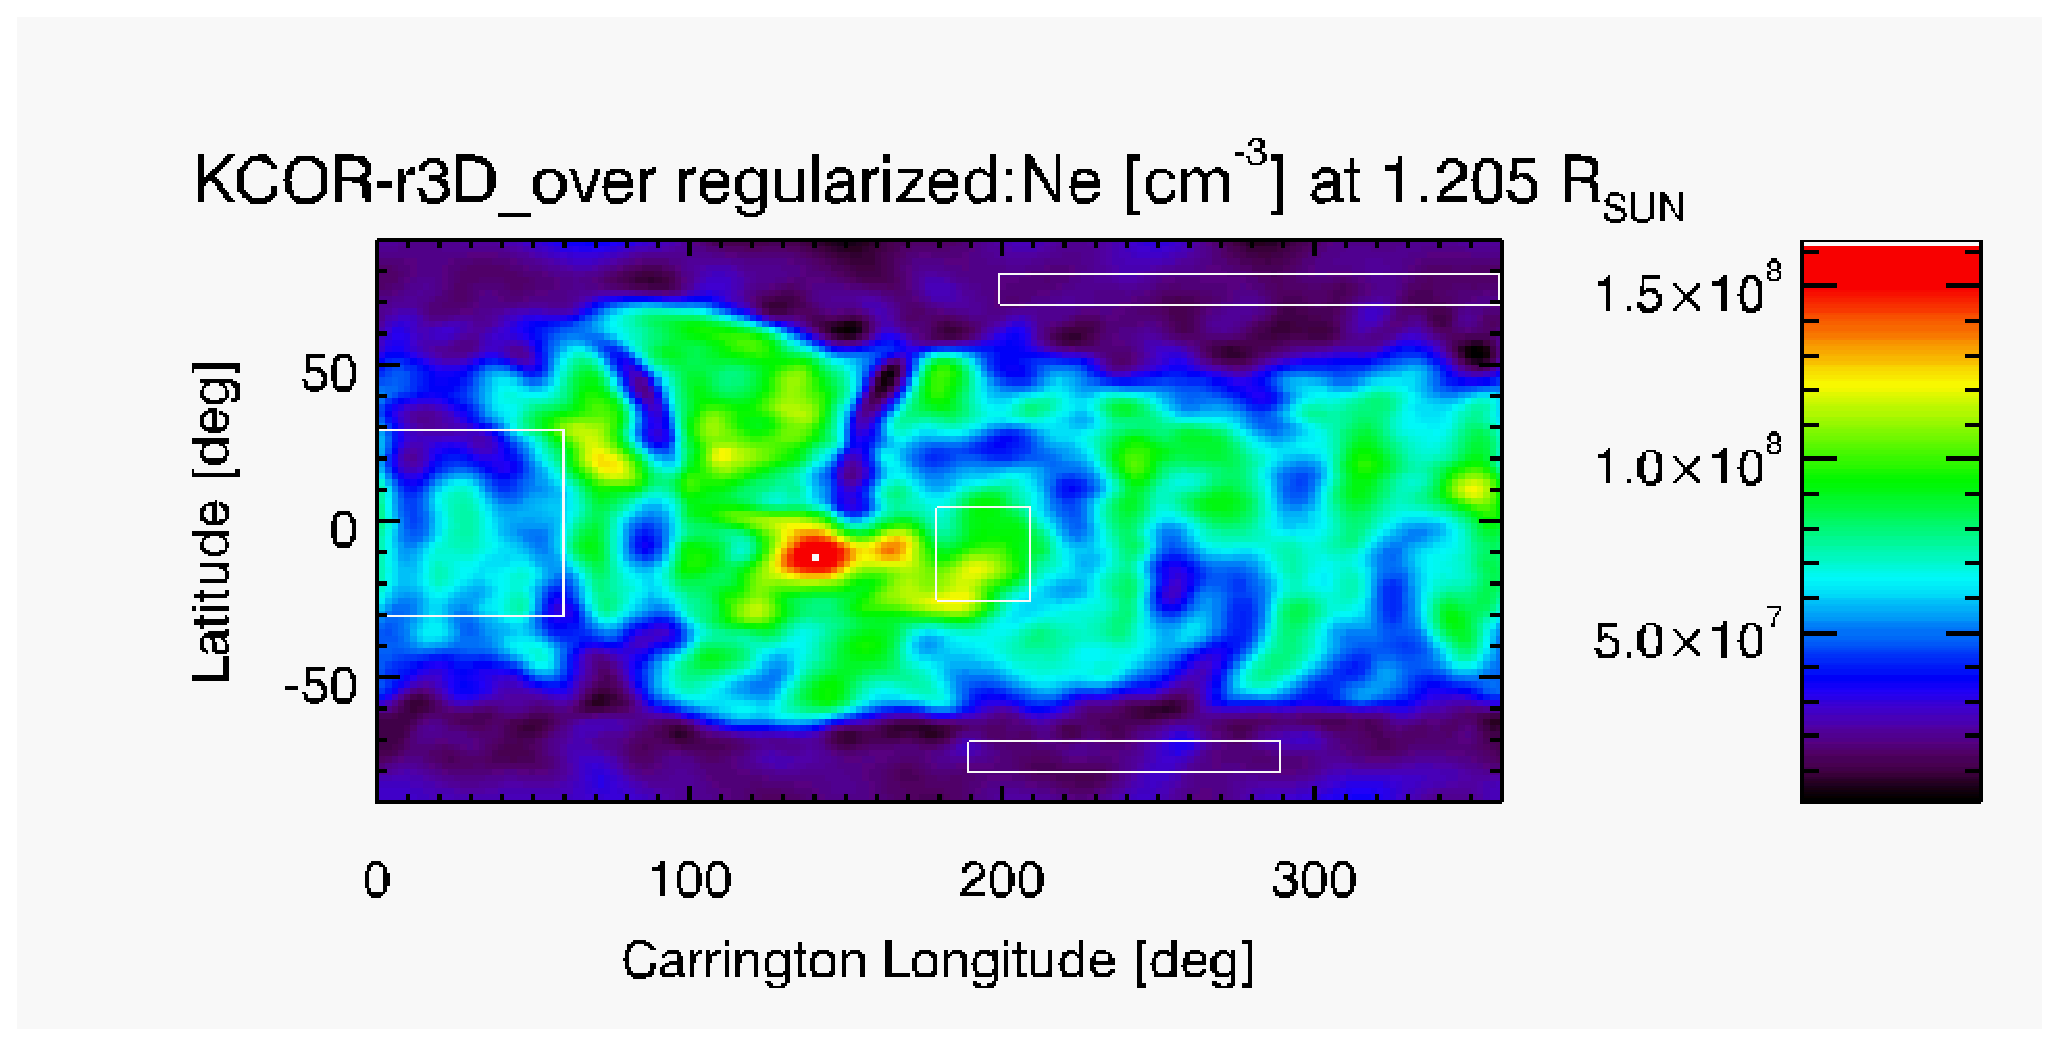
\includegraphics[height=0.34\textheight]{new_figs/map_kcor_1205.eps}
%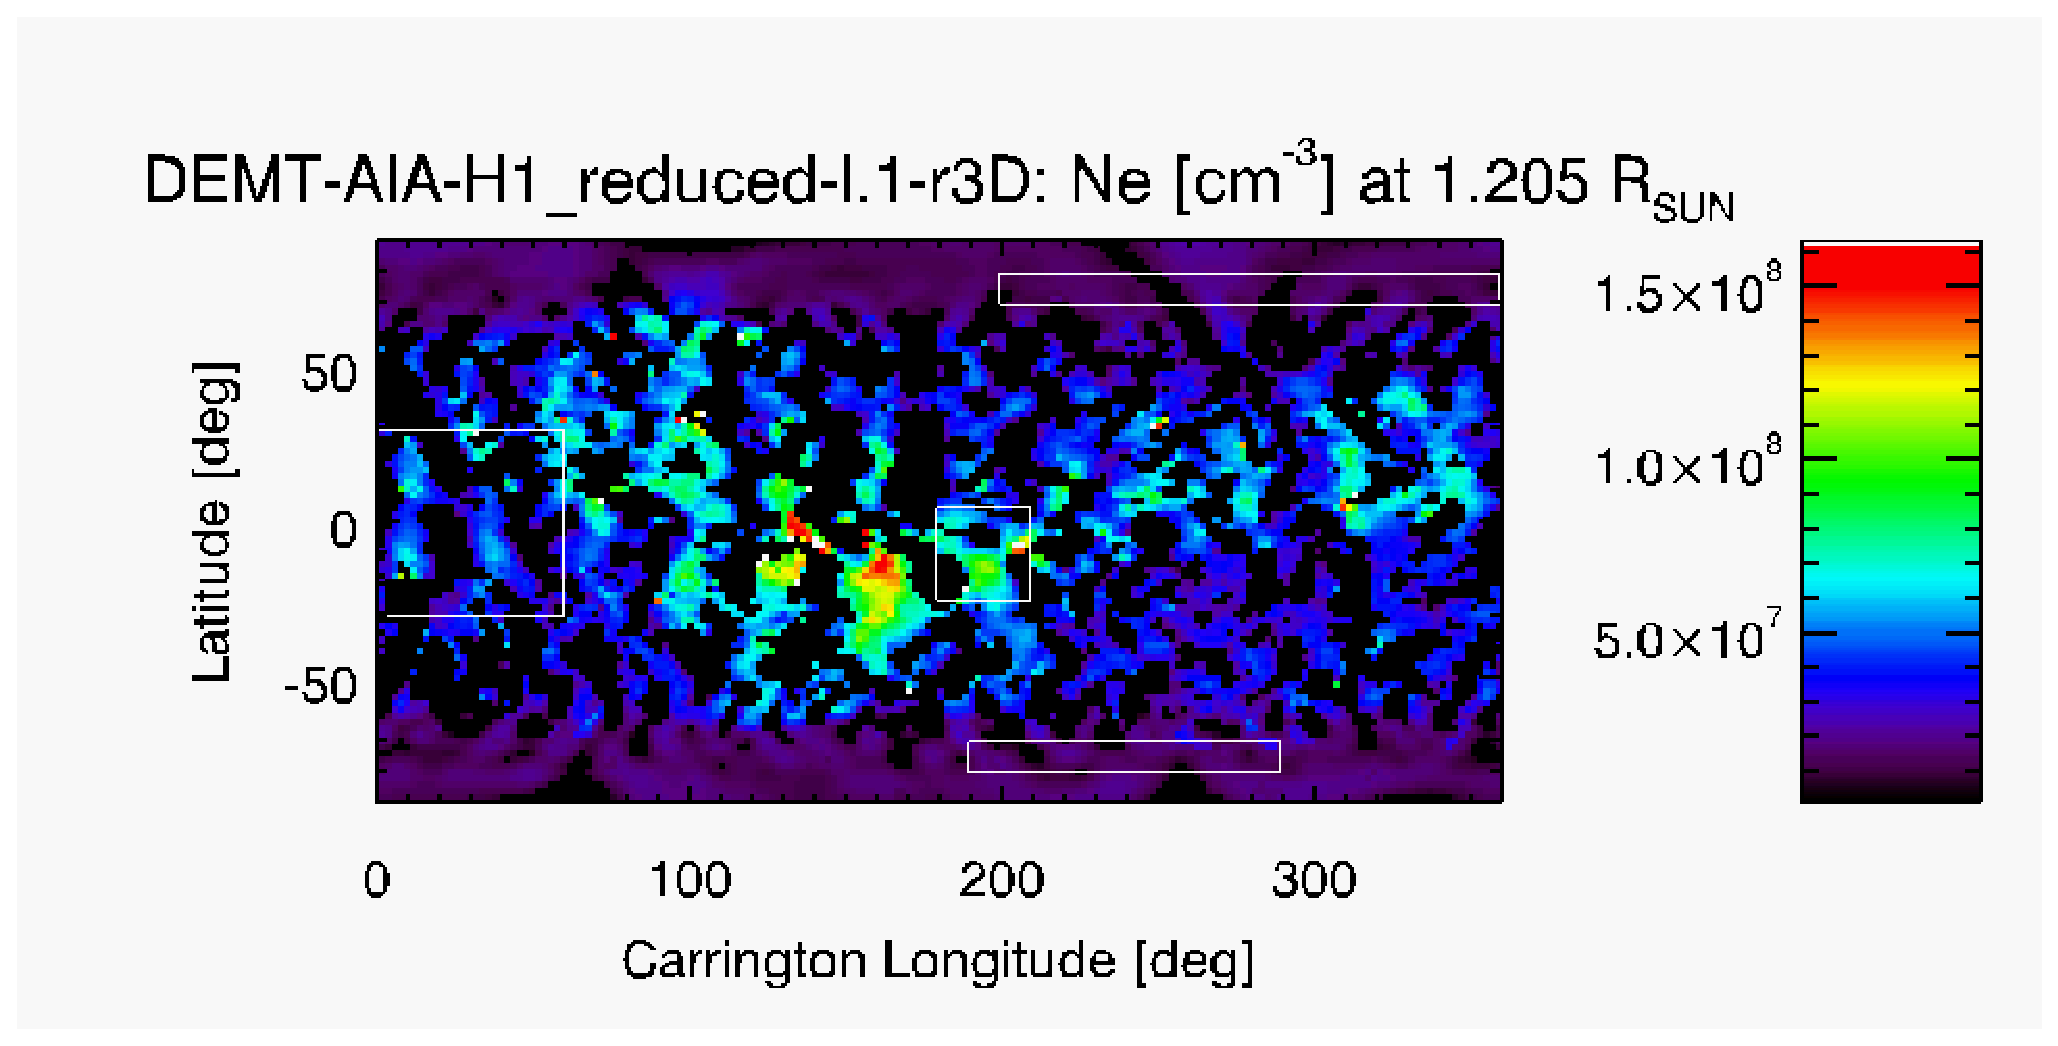
\includegraphics[height=0.34\textheight]{new_figs/map_aia_1205.eps}
}
%--------------------------------------------------
\frame{
\begin{center}
  \azul{Streamer Region}\\
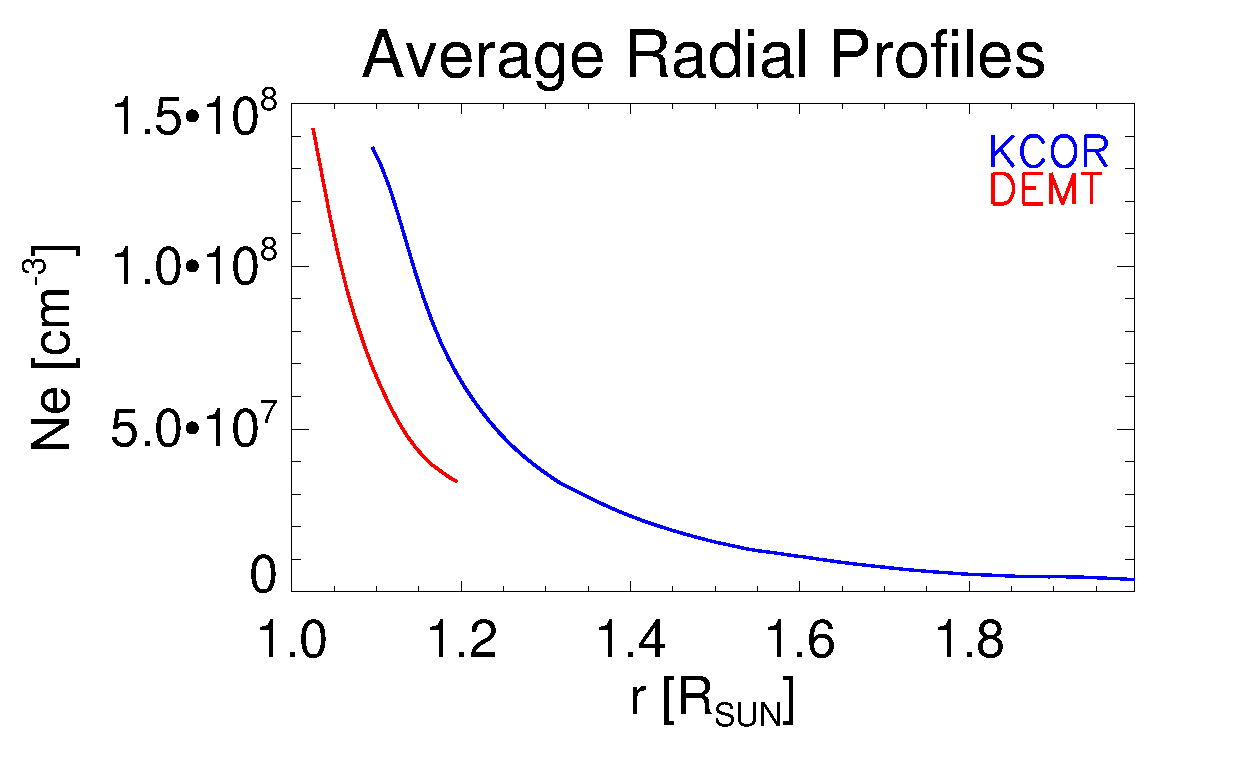
\includegraphics[height=0.26\textwidth]{new_figs/Average_Radial_Profiles_KCOR-Tom_vs_DEMT_CR2198_Hh_l45_kcor_subreg-Quiet-region1.eps}
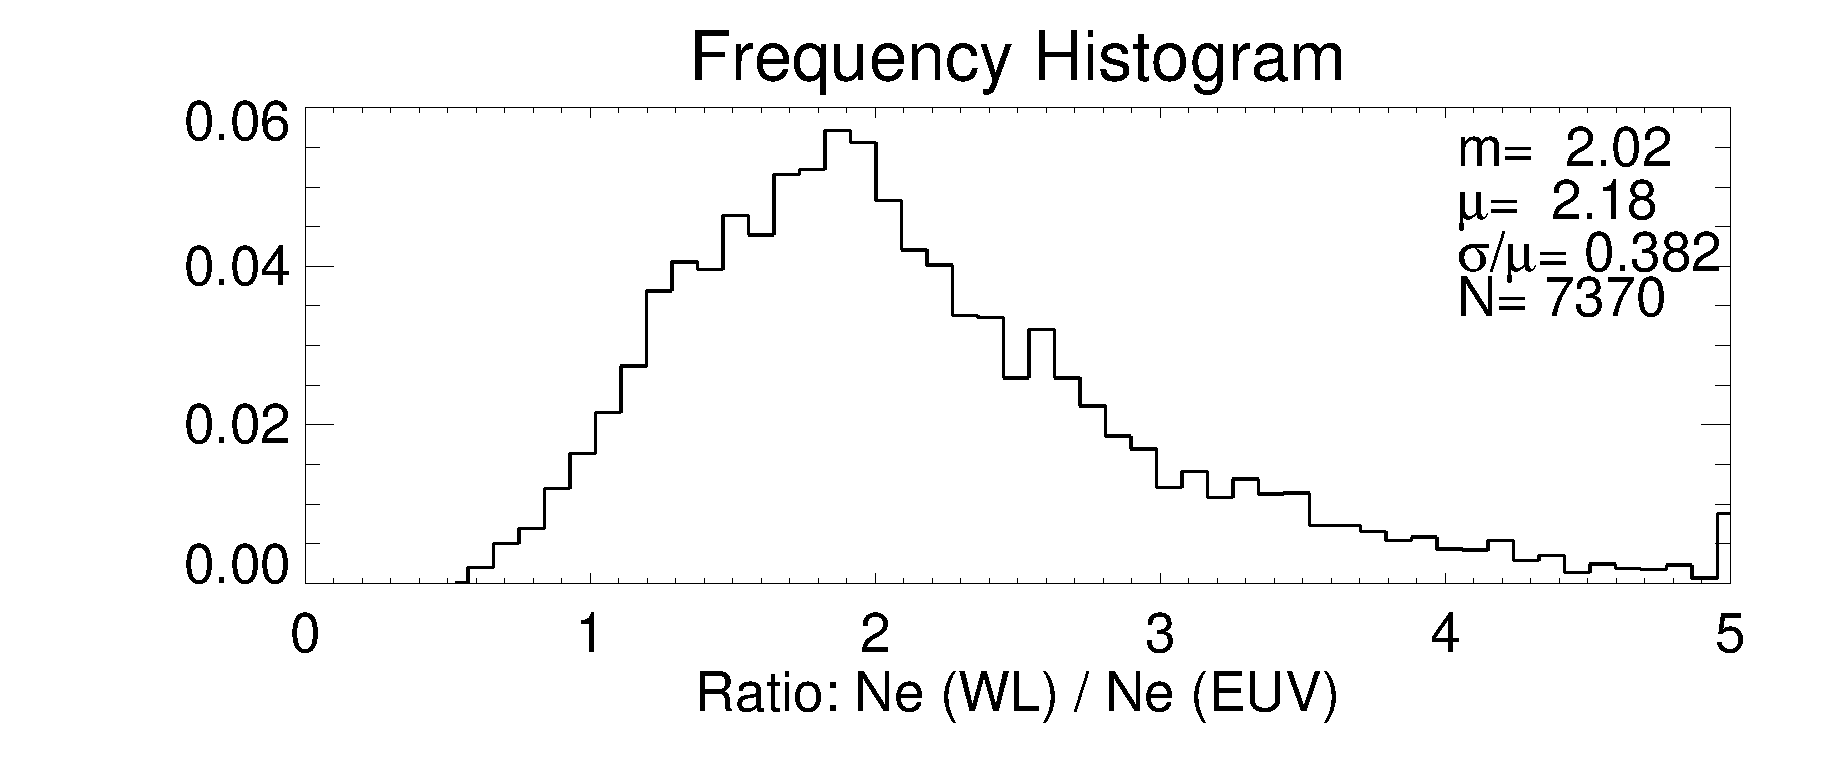
\includegraphics[height=0.26\textwidth]{new_figs/comparison_KCOR-Tom_vs_DEMT_CR2198_Hh_l45_kcor_subreg-Quiet-region1_range1105-1195_Rsun.eps}\\
\azul{Polar Region}\\
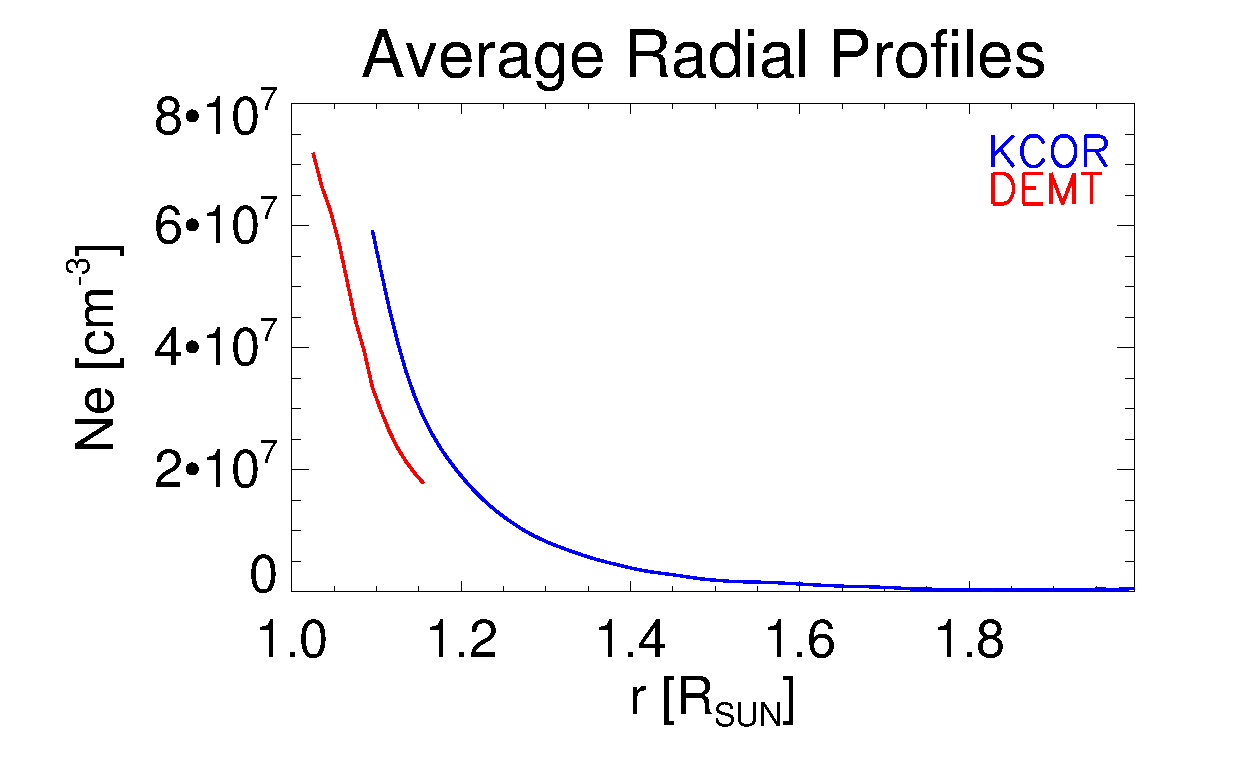
\includegraphics[height=0.26\textwidth]{new_figs/Average_Radial_Profiles_KCOR-Tom_vs_DEMT_CR2198_Hh_l45_kcor_subreg-Open-region_N.eps}
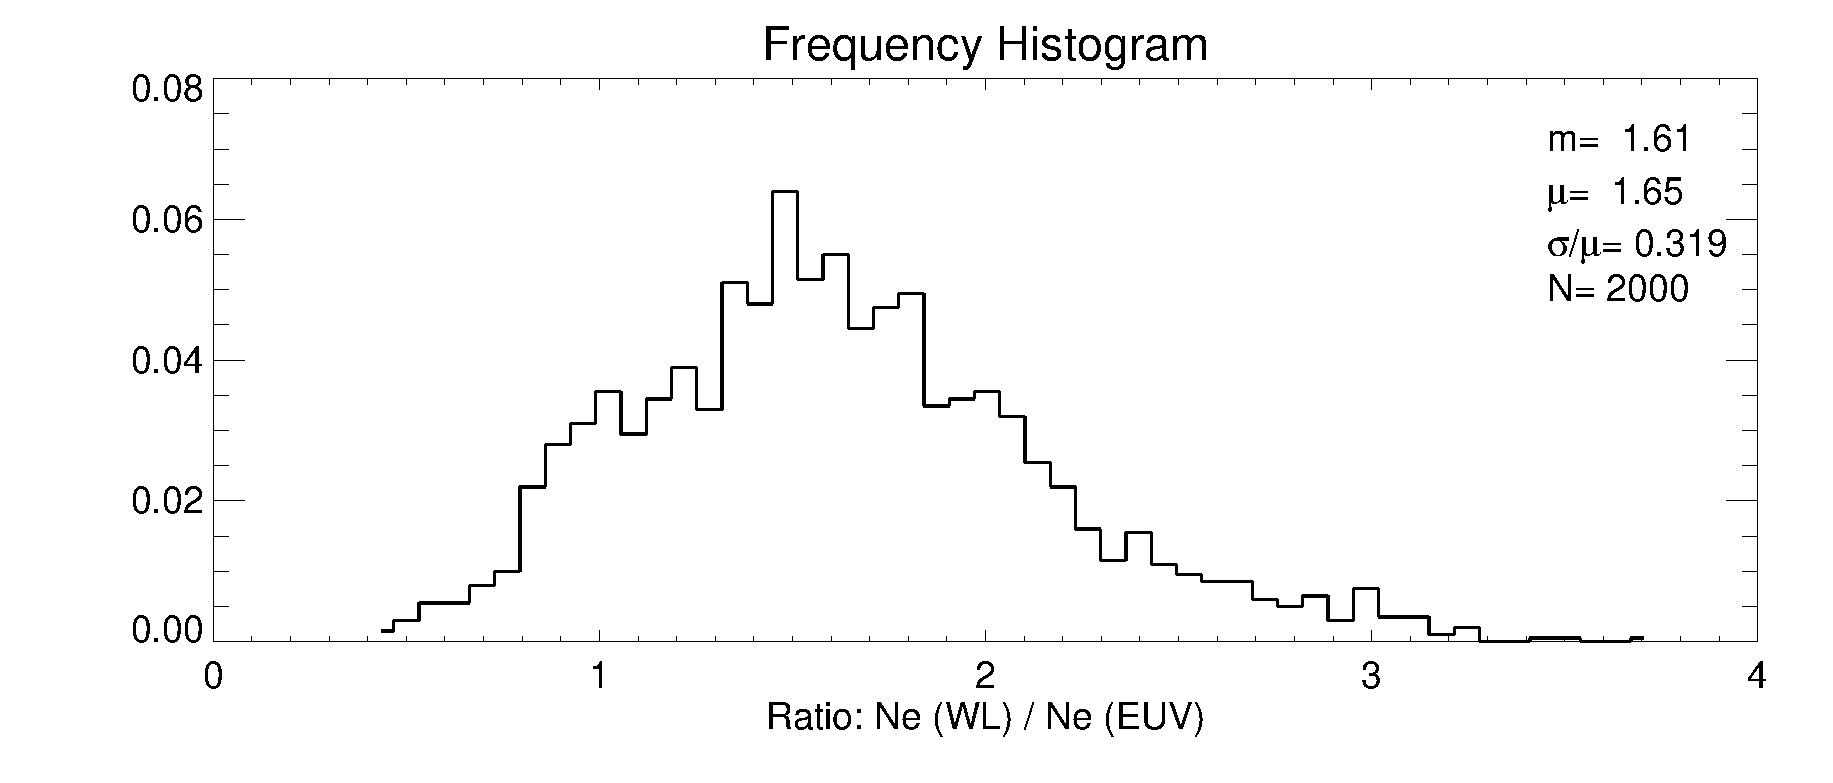
\includegraphics[height=0.26\textwidth]{new_figs/comparison_KCOR-Tom_vs_DEMT_CR2198_Hh_l45_kcor_subreg-Open-region_N_range1105-1155_Rsun.eps}
\end{center}
}
%-----------------------------

%---------------------
\frame{
\titulo{Discussion}
\vspace{-1.cm}
\begin{itemize}
 \item  $\Eeuv \propto \AvgNE2 = f\,\AvgNe^2$, where \azul{filling factor} is defined as $f\equiv\AvgNE2 / \AvgNe^2$

\item  $\Ewl \propto \AvgNe$

\item  Then: $\AvgNe_{\rm{WL}} / \AvgNe_{\rm{EUV}} \propto \sqrt{f}$

\item  If differences in the results are solely attributed to filling factor: $f\sim 2$ in open region, and $f\sim 4$ in closed region.

\item  Note that: $\SigmaNe^2 \equiv \rm{Var}N_e = \AvgNE2 - \AvgNe^2 = \AvgNe^2 \, (f-1)$

\item  So that: $\SigmaNe / \AvgNe = \sqrt{f-1}$.

\item  Where $f$ is larger (closed region) the density distribution has larger variance.
\end{itemize}
}

%-----------------------------------------
\frame{
\titulo{Future Work}
\vspace{-1.cm}
\begin{itemize}
 \item  To refine discrimination of different structures we will next trace results along field lines from MHD models.

 \item  Other factor that can explain the observed differences is [Fe].

 \item  This work (in progress) is a first step towards future implementation of \azul{Multi-Instrument Tomography (MIT)}. 

 \item  Future work: MIT aims at using tomographies in WL, EUV and also visible spectral lines (upcoming UCoMP instrument) to simultaneously derive reconstructions for the different physical parameters $\AvgNe, \SigmaNe, f, \rm{[Fe]}$, as well as $\AvgTe, \SigmaTe$. 
\end{itemize}
}
\begin{comment}
%----------------> TOMOGRAFIA <------------------------------------------------------
{
\setbeamercolor{normal text}{fg=white}
\setbeamercolor{frametitle}{fg=white}
\usebeamercolor[fg]{normal text}
\usebackgroundtemplate{\includegraphics[width=\paperwidth]{figuras/Hathaway_NASA_MSFC.eps}}
\frame{

}
}
%------------------------------------------------------------------------------------
{
\setbeamercolor{normal text}{fg=white}
\setbeamercolor{frametitle}{fg=white}
\usebeamercolor[fg]{normal text}
\usebackgroundtemplate{\includegraphics[width=\paperwidth]{figuras/orbits.eps}}
\frame{
\titulo{Full-Sun EUV Space Telescopes}
\scriptsize
\vspace{-1.75cm}
\begin{center}
%\begin{itemize}
%\item
Extreme ultraviolet Imaging Telescope {\bf (EIT)}\\ 
Solar and Heliospheric Observatory {\bf(SOHO)}\\
1996-2005. Sun-Earth L1 orbit.
%\salto
%\item
%Transition Region And Coronal Explorer \azul{(TRACE)}. 1998-2010.\\
%Sun-synchronous low Earth orbit (LEO).
\salto
%\item
Extreme UltraViolet Imager {\bf (EUVI)}\\
Solar TErrestrial RElations Observatory {\bf(STEREO)}\\ 
2007-2023. Two 1AU orbits behind and ahead Earth.
\salto
%\item
%Atmospheric Imaging Assembly {\bf (AIA)}\\ 
%Solar Dynamics Observatory {\bf(SDO)}\\ 
%2010-2020. Geosynchronic orbit around Earth.
%\end{itemize}
\end{center}
\vspace{-0.5cm}
\begin{table}[ht]
%\begin{center}
\begin{tabular}{llll}
\hline
Instrument & EIT  & EUVI \\%& AIA\\
\hline
\# Coronal Bands & 3  & 3  \\%& 6\\
Temperature range (MK) & 
[0.5,3.0] & [0.5,3.0] \\%& [0.5,15]\\
%F.O.V. (\rsun) & 2.8  & 3.4 \\% & 2.6 \\
%Image size & $1024^2$ & $2048^2$ & $4096^2$\\
%Resolution [arc sec; $10^{-3}$\rsun]  & 2.6 & 1.6 & 0.6\\
\hline
\end{tabular}
%\end{center}
\end{table}
}
}
%-------------------------------------------------------
\frame{
\titulo{Intensidad específica y pasabandas}
\footnotesize
\begin{columns}
\column{0.5\textwidth}
\begin{center}
Señal del pixel $j$ de la banda $k$\\
$ I_{k,j} = \int \mathrm{d}\lambda  \ J_j(\lambda)  \ \phi_k(\lambda) $\\
~[ph / sec]
{\includegraphics[width=0.8\linewidth]{figuras/all_wave_a.eps}}\\
Intensidad específica $J_j(\lambda)$\\
~[ph/\cmsq \,sr\,sec\,\AA]
\end{center}
\column{0.5\textwidth}
\begin{center}
Los pasabandas $\phi_k$\\
seleccionan líneas de Fe
\end{center}
{\includegraphics[width=0.99\linewidth]{figuras/euvi_bandpasses.eps}}
\begin{center}
Temperaturas características:\\
1.0, 1.5, 2.0 MK
\end{center}
\end{columns}
}
%-------------------------------------------------------------------
\frame{
\titulo{El problema tomográfico}
\footnotesize
%\begin{itemize}
%\item
%The Coronal volume is discretized over the FOV, 1.00$\rightarrow$1.25 \rsun.\\
%\azul{\# Cells:} $\azul{I}\,=\,25\times90\times180\sim\ \azul{4\times10^5}$
%\mediosalto
%Typical cell-size:\ \ 0.01\,\rsun\,$\times$ 2\deg $\times$ 2\deg \ $\sim$ \ $7\times10^3$km $\times$ %($25\times10^3$km)$^2$
%\salto
%\azul{\# Pixels:} $\azul{J}\,=\,512^2\times4\times27.5\times0.7\sim\ \azul{2\times10^7}$
%\salto
\begin{columns}
\column{0.225\textwidth}
\begin{center}
360\deg\\   
{\includegraphics[width=0.99\linewidth]
{figuras/20081117.0906.B.S1.195.norot.1024.DNSEC.DESPIKE-tn8.Norm-Ck0.rs.b4.fts.eps}}
\end{center}
\column{0.225\textwidth}
\begin{center}
270\deg\\
{\includegraphics[width=0.99\linewidth]
{figuras/20081123.2106.B.S1.195.norot.1024.DNSEC.DESPIKE-tn8.Norm-Ck0.rs.b4.fts.eps}}
\end{center}
\column{0.225\textwidth}
\begin{center}
180\deg\\
{\includegraphics[width=0.99\linewidth]
{figuras/20081130.1506.B.S1.195.norot.1024.DNSEC.DESPIKE-tn8.Norm-Ck0.rs.b4.fts.eps}}
\end{center}
\column{0.225\textwidth}
\begin{center}
90\deg\\
{\includegraphics[width=0.99\linewidth]
{figuras/20081207.0906.B.S1.195.norot.1024.DNSEC.DESPIKE-tn8.Norm-Ck0.rs.b4.fts.eps}}
\end{center}
\end{columns}
\begin{itemize}
\item
Discretizando la intensidad en cada banda $k$:
$$
\azul{I_{k,j}} = \azul{
\int_{\mathrm{LOS}} \mathrm{d}l} \ 
\rojo{FBE_k \left(\azul{\br_j(l)}\right)}
\ \ \rightarrow \ \
\azul{\bI_k} = \azul{\bL_k\,\cdotp\,} \rojo{{\bf FBE}_k} %+ \bn_k
$$
\end{itemize}

{\includegraphics[width=0.99\linewidth]
{figuras/195_otuput_tomo.eps}}
}

%-----------------------------------------------------------
\frame{
\titulo{Resultados tomográficos 3D}
\scriptsize
\begin{columns}
\column{0.35\textwidth}
\begin{center}
Emisividades de Banda (FBE)\\
\vskip 0.25cm
{\includegraphics[width=\linewidth]{figuras/FBE-EUVI-171.eps}}
{\includegraphics[width=\linewidth]{figuras/FBE-EUVI-195.eps}}
{\includegraphics[width=\linewidth]{figuras/FBE-EUVI-284.eps}}
\end{center}
\column{0.3\textwidth}
\tiny
$\azul{FBE_{k,i} }  =  \azul{\int \mathrm{d}T \  R_k(T)  \rojo{{\sf LDEM}_i(T)} }$.
\vskip 0.25cm
Tomando los momentos de la \rojo{${\sf LDEM}_i(T)$}:\\
\vskip 0.25cm
$\left< N_e^2\right>_i = \int \mathrm{d} T \ \, \rojo{{\sf LDEM}_i(T)}$\\
\vskip 0.25cm
$T_{m,i}   = \frac{1}{\left< N_e^2\right>_i } \int \mathrm{d}T\ T \ \, \rojo{{\sf LDEM}_i(T)}$\\
\vskip 0.25cm
\frame{\includegraphics[width=\linewidth]{figuras/LDEM.eps}}
\column{0.35\textwidth}
\scriptsize
\begin{center}
Densidad\\
{\includegraphics[width=\linewidth]{figuras/Ne-2081-EUVI-l075.eps}}\\
Temperatura\\
{\includegraphics[width=\linewidth]{figuras/Tm-2081-EUVI-l075.eps}}\\
$R=\frac{1}{N}\sum_{k=1}^N |1-E_{k,syn}/E_{k,tom}|$\\
{\includegraphics[width=\linewidth]{figuras/R-2081-EUVI-l075.eps}}
\end{center}
\end{columns}
}

%------------------------------------------------------------
\frame{ 
\vspace{-0.15cm}
\titulo{Magnetograma y extrapolación coronal}
\footnotesize
\begin{columns}
\column{0.5\textwidth}
\begin{center}
{\includegraphics[width=0.8\textwidth]{figuras/magnetograma_gris.eps}}
{\includegraphics[width=0.9\linewidth]{figuras/aNe.eps}}
%\begin{equation}
% N_e(r) = N_{e,1}\, \exp{[-(h/\l)/(r/\mrsun)]}
%\end{equation}
\end{center}
\column{0.5\textwidth}
\begin{center}
{\includegraphics[width=0.8\textwidth]{figuras/CR2081-PFSS.eps}}
{\includegraphics[width=0.9\linewidth]{figuras/aTm.eps}}
%\begin{equation}
% T(r) = a r + b
% \end{equation}
\end{center}
\end{columns}
}

%-------------------> 
\frame{ 
\vspace{-0.05cm}
\titulo{Comparación de mínimos}
\footnotesize
\begin{columns}
\column{0.5\textwidth}
\hfil Marzo - 2009
{\includegraphics[width=0.86\textwidth]{figuras/Ne_1105_cr2081l075_ldem_v3_errorbox_base_test.eps}}
%\hskip 0.1cm
{\includegraphics[width=0.86\textwidth]{figuras/Tm_1105_cr2081l075_ldem_v3_errorbox_base_test.eps}}\\
{\includegraphics[width=0.86\textwidth]{figuras/R_1105_cr2081l075_ldem_v3_errorbox_base_test.eps}}
\column{0.5\textwidth}
\hfil Octubre - 1996
{\includegraphics[width=0.86\textwidth]{figuras/Ne_1105_cr1915l075_ldem_v3_errorbox_base_test.eps}}
%\hskip 0.1cm
{\includegraphics[width=0.86\textwidth]{figuras/Tm_1105_cr1915l075_ldem_v3_errorbox_base_test.eps}}\\
{\includegraphics[width=0.86\textwidth]{figuras/R_1105_cr1915l075_ldem_v3_errorbox_base_test.eps}}
\end{columns}
}
%-----------------------------------------
\frame{
\titulo{Comparación Cuantitativa}
\footnotesize
\hfil Marzo - 2009 \hfil Octubre - 1996
\begin{center}
%Identification of Diverse Coronal Regions\\
{\includegraphics[width=0.49\textwidth]{figuras/Rpoint-map_1105_5colores_paper_euvi_v3.eps}}
{\includegraphics[width=0.49\textwidth]{figuras/Rpoint-map_1105_5colores_paper_eit_v3.eps}}
\vskip 0.15cm
Equatorial Streamer\\
{\includegraphics[width=0.32\textwidth]{figuras/test_compa_EUVI_EIT_newzones_todo_cap3_v1_lowlat_Nebasal.eps}}
{\includegraphics[width=0.32\textwidth]{figuras/test_compa_EUVI_EIT_newzones_todo_cap3_v1_lowlat_lambda_N.eps}}
{\includegraphics[width=0.32\textwidth]{figuras/test_compa_EUVI_EIT_newzones_todo_cap3_v1_lowlat_Te.eps}}
\vskip 0.1cm
%Southern Coronal Hole\\
%{\includegraphics[width=0.32\textwidth]{figuras/test_compa_EUVI_EIT_newzones_todo_cap3_v1_open_S_Nebasal_H.eps}}
%{\includegraphics[width=0.32\textwidth]{figuras/test_compa_EUVI_EIT_newzones_todo_cap3_v1_open_S_lambda_N_H.eps}}
%{\includegraphics[width=0.32\textwidth]{figuras/test_compa_EUVI_EIT_newzones_todo_cap3_v1_open_S_Te_H.eps}}
\end{center}
}
%--------------------------------------------

\frame{
\titulo{Estructuras de temperatura}
\footnotesize
\begin{center}
\azul{Marzo - 2009 \hskip 4cm Octubre - 1996}
\vskip 0.2cm
%Identificación de Arcos UP/DOWN\\
{\includegraphics[width=0.49\textwidth]{figuras/Rpoint_6colores_cap4_v3_loop_mapoc_EUVI_up-down_R1105_v2.eps}}
%{\includegraphics[width=0.48\textwidth]{figuras/Rpoint_6colores_cap4_v3_loop_EUVI_up-down_R1105_v2.eps}}
%\hskip 0.5cm
%{\includegraphics[width=0.48\textwidth]{figuras/Rpoint_6colores_cap4_v3_loop_EIT_up-down_R1105_v2.eps}} \ \ 
{\includegraphics[width=0.49\textwidth]{figuras/Rpoint_6colores_cap4_v3_loop_mapoc_EIT_up-down_R1105_v2.eps}}
\end{center}
(Huang et al. 2012, Nuevo et al. 2013, Schiff et al. 2016)
\vspace{-0.1cm}
\begin{center}
\red{\bf UP Loops} ($dT/dr > 0$) \hskip 2cm \azul{\bf DOWN Loops} ($dT/dr < 0$)\\
{\includegraphics[width=0.45\linewidth]{figuras/error_bar_Tm.up.eps}} 
%\hskip 0.5cm
{\includegraphics[width=0.45\linewidth]{figuras/error_bar_Tm.down.eps}}
\end{center}
}

%--------------------------------------------------------
%\frame{ 
%\vspace{-0.35cm}
%\titulo{Analysis of Systematic Uncertainties}
%\footnotesize
%\begin{center}
%\vskip 0.25cm
%xample: Point-Spread-Function of the EUV Detectors.
%vskip 0.25cm
%Lunar Transit without / with PSF Deconvolution.\\
%{\includegraphics[width=0.48\textwidth]{figuras/lunar_transit.eps}}
%{\includegraphics[width=0.48\textwidth]{figuras/deconvolved.eps}}
%\vskip 0.25cm
%Analysis of its Effect on Tomographic Reconstructions:\\
%{\includegraphics[width=0.32\textwidth]{figuras/compa_decon_nodecon_lowlat_Nebasal.eps}}
%{\includegraphics[width=0.32\textwidth]{figuras/compa_decon_nodecon_lowlat_lambda_N.eps}}
%{\includegraphics[width=0.32\textwidth]{figuras/compa_decon_nodecon_lowlat_Te.eps}}
%\end{center}
%}

%---------------------------------------------------------------
\frame{ 
\vspace{-0.15cm}
\titulo{Conclusiones}
\footnotesize
\begin{itemize}
\item
Propagación de incertezas sistemáticas en los resultados de la técnica tomográfica:
1) Deconvolución de la PSF - EUV\\
2) Incertezas de calibración radiométrica\\
3) Incertezas en el nivel de regularización\\
\salto
\item El último mínimo fue menos denso y mas frío que el previo.
%The last minimum was less dense and cooler than the previous one.
\salto
\item El Streamer equatorial durante el último mínimo fue mas consistente con equilibrio hidostático isotérmico.
%The equatorial Streamer during the last minimum was more consistent with isothermal hydrostatic equilibrium.
\item
\salto
Hay presencia de loops down en ambos mínimos, siendo mas dominantes en el último y distribuidos de forma mas homogénea.
%Down loops are present in both minima, being more dominating in the last one as well as distributed in a more homogeneous fashion.


%Comprehensive propagation of systematic uncertainties into DEMT results:\\
%1) PSF-EUV deconvolution.\\
%2) EUV Radiometric calibration uncertainty.\\
%3) Tomography regularization level uncertainty.

\end{itemize}
}

%----------------------------------

\frame{
\titulo{Planes futuros}
\footnotesize
      \begin{itemize}
      \item Publicar los resultados de la Comparación de mínimos.
      \salto
       \item Estudio comparativo de ciclos solares utilizando tomografía en luz blanca.\\
       %Comparative study of solar cycles using WL tomography.\\
       \salto
       \item Estudio de validación sistemática de modelo MHD Space Weather Modeling Framework(SWMF).\\
       %Systematic validation study of MHD models, Space Weather Modeling Framework (SWMF).
       \salto       
     % \item Models have to account for observed differences between the two periods. Validation studies of MHD models are planned.
       
      
      \end{itemize}
}
\iffalse
\fi
\end{comment}
\end{document}

% Slides extra
